%\VignetteIndexEntry{CaseStudy}
%\VignetteEncoding{UTF-8}

\documentclass[a4paper, 11pt]{article}\usepackage[]{graphicx}\usepackage[]{color}
% maxwidth is the original width if it is less than linewidth
% otherwise use linewidth (to make sure the graphics do not exceed the margin)
\makeatletter
\def\maxwidth{ %
  \ifdim\Gin@nat@width>\linewidth
    \linewidth
  \else
    \Gin@nat@width
  \fi
}
\makeatother

\definecolor{fgcolor}{rgb}{0.345, 0.345, 0.345}
\newcommand{\hlnum}[1]{\textcolor[rgb]{0.686,0.059,0.569}{#1}}%
\newcommand{\hlstr}[1]{\textcolor[rgb]{0.192,0.494,0.8}{#1}}%
\newcommand{\hlcom}[1]{\textcolor[rgb]{0.678,0.584,0.686}{\textit{#1}}}%
\newcommand{\hlopt}[1]{\textcolor[rgb]{0,0,0}{#1}}%
\newcommand{\hlstd}[1]{\textcolor[rgb]{0.345,0.345,0.345}{#1}}%
\newcommand{\hlkwa}[1]{\textcolor[rgb]{0.161,0.373,0.58}{\textbf{#1}}}%
\newcommand{\hlkwb}[1]{\textcolor[rgb]{0.69,0.353,0.396}{#1}}%
\newcommand{\hlkwc}[1]{\textcolor[rgb]{0.333,0.667,0.333}{#1}}%
\newcommand{\hlkwd}[1]{\textcolor[rgb]{0.737,0.353,0.396}{\textbf{#1}}}%
\let\hlipl\hlkwb

\usepackage{framed}
\makeatletter
\newenvironment{kframe}{%
 \def\at@end@of@kframe{}%
 \ifinner\ifhmode%
  \def\at@end@of@kframe{\end{minipage}}%
  \begin{minipage}{\columnwidth}%
 \fi\fi%
 \def\FrameCommand##1{\hskip\@totalleftmargin \hskip-\fboxsep
 \colorbox{shadecolor}{##1}\hskip-\fboxsep
     % There is no \\@totalrightmargin, so:
     \hskip-\linewidth \hskip-\@totalleftmargin \hskip\columnwidth}%
 \MakeFramed {\advance\hsize-\width
   \@totalleftmargin\z@ \linewidth\hsize
   \@setminipage}}%
 {\par\unskip\endMakeFramed%
 \at@end@of@kframe}
\makeatother

\definecolor{shadecolor}{rgb}{.97, .97, .97}
\definecolor{messagecolor}{rgb}{0, 0, 0}
\definecolor{warningcolor}{rgb}{1, 0, 1}
\definecolor{errorcolor}{rgb}{1, 0, 0}
\newenvironment{knitrout}{}{} % an empty environment to be redefined in TeX

\usepackage{alltt}
\usepackage[utf8]{inputenc}
\usepackage{amsmath} % e.g. for \text{} in math
\usepackage[T1]{fontenc}
\usepackage{geometry}
  \geometry{verbose,tmargin=2cm,bmargin=2cm,lmargin=2cm,rmargin=2cm}
  \setcounter{secnumdepth}{3}
  \setcounter{tocdepth}{3}
\usepackage[ttscale=0.85]{libertine}
\usepackage{makeidx}
  \makeindex
\usepackage{natbib}
\usepackage{url}
\usepackage[unicode=true,pdfusetitle,
 bookmarks=true,bookmarksnumbered=true,bookmarksopen=true,bookmarksopenlevel=2,
 breaklinks=true,pdfborder={0 0 1},backref=page,colorlinks=false, hidelinks]
 {hyperref}
\usepackage{breakurl}
\usepackage{titlesec} % for titleformat
\usepackage[nottoc]{tocbibind} % include reference in table of content
\usepackage{wrapfig}
\usepackage[dvipsnames]{xcolor}
	\definecolor{DarkGreen}{rgb}{0, .1, 0}
	\color{DarkGreen}

%%%%%%%%%%%%%%%%%%%%%%%%%%%%%% User specified LaTeX commands.
% % % % % % %  section numbering onto margins % % % %
\newlength\mylensection
\setlength\mylensection{\dimexpr\oddsidemargin+1.5cm+\hoffset\relax}
\titleformat{\section}{\normalfont\Large\itshape}{\llap{\hspace*{-\mylensection}\textcolor{YellowGreen}{\textbf{\LARGE{ \thesection}}}\hfill}}{0em}{} %

\newlength\mylensubsection
\setlength\mylensubsection{\dimexpr\oddsidemargin+1.5cm+\hoffset\relax}
\titleformat{\subsection}{\normalfont\large\itshape}{\llap{\hspace*{-\mylensubsection}\textcolor{YellowGreen}{\textbf{\Large{ \thesubsection}}}\hfill}}{0em}{} %

\newlength\mylensubsubsection
\setlength\mylensubsubsection{\dimexpr\oddsidemargin+1.2cm+\hoffset\relax}
\titleformat{\subsubsection}{\normalfont\large\itshape}{\llap{\hspace*{-\mylensubsubsection}\textcolor{YellowGreen}{\textbf{\Large{ \thesubsubsection}}}\hfill}}{0em}{} %


\renewcommand{\textfraction}{0.05}
\renewcommand{\topfraction}{0.8}
\renewcommand{\bottomfraction}{0.8}
\renewcommand{\floatpagefraction}{0.75}

\newcommand{\package}[1]{\textbf{#1}}
\newcommand{\proglang}[1]{\textsl{#1}}
\newcommand{\code}[1]{\texttt{#1}}
\newcommand{\ind}[1]{#1\index{#1}}           			   % \ind{bla} instead of bla\index{bla}
\newcommand{\indE}[1]{\emph{#1}\index{#1@\emph{#1}}}       % dito for emphasised words (e.g. English)
\newcommand{\indR}[1]{\texttt{#1}\index{#1@\texttt{#1}}}   % dito for typewriter


\renewcommand{\vec}[1]{\mathbf{#1}}                   % replaces the arrow over vectors by bold-print

\setlength{\parindent}{0pt}


\frenchspacing % avoid long spaces after a "."
\IfFileExists{upquote.sty}{\usepackage{upquote}}{}
\begin{document}

\title{A quick guide on how to use tapnet}

\author{Carsten F. Dormann}
%\thanks{\href{mailto:carsten.dormann@biom.uni-freiburg.de}{carsten.dormann@biom.uni-freiburg.de}}

\maketitle






\begin{abstract}
\noindent This document presents the case study of Benadi et al. (2021), using the data of Tinoco et al. (2017). It thereby also serves as tutorial for the use of the ``tapnet'' package.
\end{abstract}

\tableofcontents

\bigskip

\bigskip

This supplement presents the workflow for the case study. It may also serve as tutorial for the use of tapnet functions.

\textbf{References}\\
Benadi, G., Dormann, C.F., Fründ, J., Stephan, R.\& Vázquez, D.P. (2021) Quantitative prediction of interactions in bipartite networks based on traits, abundances, and phylogeny. \emph{The American Naturalist}, in press. \\
Tinoco, B.A, Graham, C.H., Aguilar, J.M. \& Schleuning, M. (2017) \emph{Oikos} 126, 52--60. DOI: 10.1111/oik.02998

%############################################## 
\clearpage
\section{Data preparation}
\begin{knitrout}\small
\definecolor{shadecolor}{rgb}{0.969, 0.969, 0.969}\color{fgcolor}\begin{kframe}
\begin{alltt}
\hlkwd{library}\hlstd{(tapnet)}
\hlkwd{data}\hlstd{(Tinoco)}
\end{alltt}
\end{kframe}
\end{knitrout}

First, we have to put all information into a single `tapnet' object, using \code{make\_tapnet}:
\begin{knitrout}\small
\definecolor{shadecolor}{rgb}{0.969, 0.969, 0.969}\color{fgcolor}\begin{kframe}
\begin{alltt}
\hlcom{# Produce tapnet objects using each network separately (1=Forest, 2=shrub, 3=cattle farm)}
\hlstd{tapnet_web1} \hlkwb{<-} \hlkwd{make_tapnet}\hlstd{(}\hlkwc{tree_low} \hlstd{= plant_tree,} \hlkwc{tree_high} \hlstd{= humm_tree,}
                           \hlkwc{networks} \hlstd{= networks[}\hlnum{1}\hlstd{],} \hlkwc{traits_low} \hlstd{= plant_traits,}
                           \hlkwc{traits_high} \hlstd{= humm_traits,} \hlkwc{abun_low}\hlstd{=plant_abun[}\hlnum{1}\hlstd{],}
                           \hlkwc{abun_high}\hlstd{=humm_abun[}\hlnum{1}\hlstd{],} \hlkwc{npems_lat} \hlstd{=} \hlnum{4}\hlstd{)}
\hlstd{tapnet_web2} \hlkwb{<-} \hlkwd{make_tapnet}\hlstd{(}\hlkwc{tree_low} \hlstd{= plant_tree,} \hlkwc{tree_high} \hlstd{= humm_tree,}
                           \hlkwc{networks} \hlstd{= networks[}\hlnum{2}\hlstd{],} \hlkwc{traits_low} \hlstd{= plant_traits,}
                           \hlkwc{traits_high} \hlstd{= humm_traits,} \hlkwc{abun_low}\hlstd{=plant_abun[}\hlnum{2}\hlstd{],}
                           \hlkwc{abun_high}\hlstd{=humm_abun[}\hlnum{2}\hlstd{],} \hlkwc{npems_lat} \hlstd{=} \hlkwa{NULL}\hlstd{)}
\end{alltt}
\end{kframe}
\end{knitrout}
Note: 

(a) We use only 4 phylogenetic eigenvectors (PEMs, for ``maps'', and because PE is too short to be unambiguous) for the first network, but all for the other two for evaluation. The ``value'' NULL enforces the use of all PEMs.

(b) Because each web has only some species present, some PEMs will automatically be dropped (those relevant only for the missing species). As a consequence, web2 may now \textbf{not} have the same PEMs used for web1 (which are required for prediction from web1 to web 2). Let's check:

\begin{knitrout}\small
\definecolor{shadecolor}{rgb}{0.969, 0.969, 0.969}\color{fgcolor}\begin{kframe}
\begin{alltt}
\hlkwd{colnames}\hlstd{(tapnet_web1}\hlopt{$}\hlstd{networks[[}\hlnum{1}\hlstd{]]}\hlopt{$}\hlstd{pems}\hlopt{$}\hlstd{low)} \hlcom{# names of fitted PEMs}
\end{alltt}
\begin{verbatim}
## [1] "V_1" "V_2" "V_3" "V_7"
\end{verbatim}
\begin{alltt}
\hlkwd{colnames}\hlstd{(tapnet_web1}\hlopt{$}\hlstd{networks[[}\hlnum{1}\hlstd{]]}\hlopt{$}\hlstd{pems}\hlopt{$}\hlstd{high)}
\end{alltt}
\begin{verbatim}
## [1] "V_1" "V_3" "V_6" "V_8"
\end{verbatim}
\begin{alltt}
\hlkwd{colnames}\hlstd{(tapnet_web2}\hlopt{$}\hlstd{networks[[}\hlnum{1}\hlstd{]]}\hlopt{$}\hlstd{pems}\hlopt{$}\hlstd{low)} \hlcom{# names of PEMs all present }
\end{alltt}
\begin{verbatim}
##  [1] "V_1"  "V_2"  "V_3"  "V_5"  "V_7"  "V_8"  "V_10" "V_11" "V_16" "V_19"
## [11] "V_20" "V_21" "V_22" "V_25" "V_27" "V_28"
\end{verbatim}
\begin{alltt}
\hlkwd{colnames}\hlstd{(tapnet_web2}\hlopt{$}\hlstd{networks[[}\hlnum{1}\hlstd{]]}\hlopt{$}\hlstd{pems}\hlopt{$}\hlstd{high)} \hlcom{# V_8 (high) is missing!}
\end{alltt}
\begin{verbatim}
## [1] "V_1"  "V_3"  "V_4"  "V_6"  "V_7"  "V_9"  "V_11" "V_12" "V_13"
\end{verbatim}
\end{kframe}
\end{knitrout}
We can see that for the lower level, all PEMs were computed for web2, but not for the higher level, where \code{V\_8} is missing. We compute that, using the helper function \code{pems\_from\_tree}, and add it to the tapnet-object. (Because this function is not exported, we need to use the triple-colon when calling it explicitly from the package.) Then we do the same with web3.
\begin{knitrout}\small
\definecolor{shadecolor}{rgb}{0.969, 0.969, 0.969}\color{fgcolor}\begin{kframe}
\begin{alltt}
\hlstd{tapnet_web2}\hlopt{$}\hlstd{networks[[}\hlnum{1}\hlstd{]]}\hlopt{$}\hlstd{pems}\hlopt{$}\hlstd{high}\hlopt{$}\hlstd{V_8} \hlkwb{<-} \hlstd{tapnet}\hlopt{:::}\hlkwd{pems_from_tree}\hlstd{(humm_tree)[}\hlkwd{colnames}\hlstd{(}
  \hlstd{tapnet_web2}\hlopt{$}\hlstd{networks[[}\hlnum{1}\hlstd{]]}\hlopt{$}\hlstd{web),} \hlstr{"V_8"}\hlstd{]}
\hlkwd{colnames}\hlstd{(tapnet_web2}\hlopt{$}\hlstd{networks[[}\hlnum{1}\hlstd{]]}\hlopt{$}\hlstd{pems}\hlopt{$}\hlstd{high)} \hlcom{# check: complete!}
\end{alltt}
\begin{verbatim}
##  [1] "V_1"  "V_3"  "V_4"  "V_6"  "V_7"  "V_9"  "V_11" "V_12" "V_13" "V_8"
\end{verbatim}
\end{kframe}
\end{knitrout}
Using the \code{colnames(.)}-line we can check that they are now complete (not shown).

As an additional preliminary step, we may want to check for correlation between the phylogenetic eigenvectors and the observed traits:
\begin{knitrout}\small
\definecolor{shadecolor}{rgb}{0.969, 0.969, 0.969}\color{fgcolor}\begin{kframe}
\begin{alltt}
\hlkwd{cor}\hlstd{(}\hlkwd{cbind}\hlstd{(tapnet_web1}\hlopt{$}\hlstd{networks[[}\hlnum{1}\hlstd{]]}\hlopt{$}\hlstd{pems}\hlopt{$}\hlstd{low, tapnet_web1}\hlopt{$}\hlstd{networks[[}\hlnum{1}\hlstd{]]}\hlopt{$}\hlstd{traits}\hlopt{$}\hlstd{low))}
\end{alltt}
\begin{verbatim}
##                           V_1         V_2         V_3         V_7
## V_1                1.00000000 -0.03323508  0.19929407  0.01950265
## V_2               -0.03323508  1.00000000 -0.02390179  0.02484880
## V_3                0.19929407 -0.02390179  1.00000000  0.02538867
## V_7                0.01950265  0.02484880  0.02538867  1.00000000
## Corolla_length_mm  0.30147805 -0.14321786  0.23301956 -0.40838875
##                   Corolla_length_mm
## V_1                       0.3014780
## V_2                      -0.1432179
## V_3                       0.2330196
## V_7                      -0.4083887
## Corolla_length_mm         1.0000000
\end{verbatim}
\begin{alltt}
\hlkwd{cor}\hlstd{(}\hlkwd{cbind}\hlstd{(tapnet_web1}\hlopt{$}\hlstd{networks[[}\hlnum{1}\hlstd{]]}\hlopt{$}\hlstd{pems}\hlopt{$}\hlstd{high, tapnet_web1}\hlopt{$}\hlstd{networks[[}\hlnum{1}\hlstd{]]}\hlopt{$}\hlstd{traits}\hlopt{$}\hlstd{high))}
\end{alltt}
\begin{verbatim}
##                            V_1         V_3         V_6         V_8
## V_1                  1.0000000 -0.21978007 -0.11948531 -0.14519738
## V_3                 -0.2197801  1.00000000  0.07786362  0.01687728
## V_6                 -0.1194853  0.07786362  1.00000000  0.28972218
## V_8                 -0.1451974  0.01687728  0.28972218  1.00000000
## Bill_length_mean_mm  0.5839393  0.23682088  0.10121502 -0.28068808
##                     Bill_length_mean_mm
## V_1                           0.5839393
## V_3                           0.2368209
## V_6                           0.1012150
## V_8                          -0.2806881
## Bill_length_mean_mm           1.0000000
\end{verbatim}
\end{kframe}
\end{knitrout}
In this case, correlations are moderate ($-0.4$ for the strongest lower-level and $0.58$ for the higher-level traits) and indicate some phylogenetic signal in the observed trait. Note, however, that latent traits are linear combinations of phylogenetic traits and this correlation does not check for collinearity with such a construct. We shall do that after fitting.


\section{Fit web1 using the tapnet approach}
We here assume that all trait matches are best described using a normal distribution. Alternatively, we could use the shifted log-normal. Next, we evaluate the goodness-of-fit of this fit:
\begin{knitrout}\small
\definecolor{shadecolor}{rgb}{0.969, 0.969, 0.969}\color{fgcolor}\begin{kframe}
\begin{alltt}
\hlstd{fit_web1} \hlkwb{<-} \hlkwd{fit_tapnet}\hlstd{(}\hlkwc{tapnet} \hlstd{= tapnet_web1,} \hlkwc{method}\hlstd{=}\hlstr{"SANN"}\hlstd{)} \hlcom{# very slow, but reliable}
\hlcom{#fit_web1 <- fit_tapnet(tapnet = tapnet_web1) # the default way}
\hlcom{#fit_web1ln <- fit_tapnet(tapnet = tapnet_web1, tmatch_type_obs = "shiftlnorm", }
\hlcom{#                         ini=fit_web1$opt$par*2) # requires some tempering with ini}
\hlstd{gof_web1_norm} \hlkwb{<-} \hlkwd{gof_tapnet}\hlstd{(fit_web1)}
\hlstd{gof_web1_norm}
\end{alltt}
\begin{verbatim}
## $bc_sim_web
## [1] 0.4700434
## 
## $cor_web
## [1] 0.506687
## 
## $net_indices
## $net_indices[[1]]
##           Index   Observed       Mean     Median       q2.5      q97.5
## 1   connectance  0.3250000  0.6944528  0.6917293  0.6041667  0.7857143
## 2          NODF 62.5076453 75.9450699 76.1949456 68.5033638 81.9754513
## 3 weighted NODF 39.1972477 54.5116352 54.7724833 45.5104924 61.8013420
## 4            H2  0.4496136  0.1386368  0.1381887  0.1166049  0.1601014
\end{verbatim}
\end{kframe}
\end{knitrout}
%Note that not every run of \code{fit\_tapnet} will be successful; many start with poor choice of initial parameters and hence throw an error message. This is something we still have to work on.

The goodness-of-fit function returns the similarity between fitted and observed network expressed as Bray-Curtis similarity (\code{bc\_sim\_web}), where 0.50 is not a bad value; as the correlation between fitted and observed number of interactions, expressed as Spearman correlation (\code{cor\_web}), which is our key comparison criterion at 0.52; and, finally, some selected network indices were computed for the observed and repeated draws from the fitted multinomial distribution. In this case, none of the four indices includes the observed even in the 95\% confidence interval (i.e. not good).

We can also have a look at the fitted model parameters:
\begin{knitrout}\small
\definecolor{shadecolor}{rgb}{0.969, 0.969, 0.969}\color{fgcolor}\begin{kframe}
\begin{alltt}
\hlstd{fit_web1}
\end{alltt}
\begin{verbatim}
## $par_opt
## $par_opt$lat_low
##         V_1         V_2         V_3         V_7 
##  2.64756311  4.43496460 -0.08270909 -1.13704950 
## 
## $par_opt$lat_high
##        V_1        V_3        V_6        V_8 
##  5.2243635  2.9772795 -0.4693686  1.1060889 
## 
## $par_opt$pem_shift
##   pem_shift 
## -0.04238474 
## 
## $par_opt$tmatch_width_pem
## tmatch_width_pem 
##        0.4641643 
## 
## $par_opt$tmatch_width_obs
## tmatch_width_obs1 
##          6.093618 
## 
## $par_opt$delta
##     delta 
## 0.0156301 
## 
## 
## $tmatch_type_pem
## [1] "normal"
## 
## $tmatch_type_obs
## [1] "normal"
## 
## $lambda
## [1] 0
## 
## $method
## [1] "SANN"
## 
## $maxit
## [1] 50000
## 
## $opt
## $opt$par
##               V_1               V_2               V_3               V_7 
##        0.97363964        4.43496460       -0.08270909       -1.13704950 
##               V_1               V_3               V_6               V_8 
##        5.22436353        2.97727948       -0.46936861        1.10608885 
##         pem_shift  tmatch_width_pem tmatch_width_obs1             delta 
##       -0.04238474       -0.76751674        1.80724201       -4.14280305 
## 
## $opt$value
## [1] 1368.485
## 
## $opt$counts
## function gradient 
##    50000       NA 
## 
## $opt$convergence
## [1] 0
## 
## $opt$message
## NULL
## 
## 
## attr(,"class")
## [1] "fitted.tapnet"
## attr(,"tapnet_name")
## [1] "tapnet_web1"
\end{verbatim}
\end{kframe}
\end{knitrout}
The output is a bit confusing, as it contains the fitted parameters twice: first, under \code{par\_opt} in the interpretable form, i.e. back-transformed for those parameters that were constraint (PEM 1, the standard deviations of the trait-matching function and $\delta$); then again, under \code{opt}, in their untransformed form, as spit out by \code{optim}.

At least two things are interesting here:
\begin{enumerate}
  \item The standard deviation of the trait-matching function (the normal, in this case) for the observed traits is rather wide (at 7.6, see \code{par\_opt\$tmatch\_width\_obs}). Typically, this indicates that the traits were not fitting very well to each other and the model did not find the observed traits useful. (We have seen much worse, with values > 1000, though.)
  \item The value of $\delta$ is (practically) 1. A value of 1 indicates that traits (observed and latent) are as important as the abundance.
  \item Putting the two previous points together: this model hinges on the matching of the phylogenetic-informed latent traits. One reason may be that the phylogenies code up the effect of the traits, so that the trait has no remaining additional effect. Parameter \code{lambda} imposes a shrinkage to prioritise the observed trait effect over the latent traits. (Imposing some shrinkge, e.g. setting \code{lambda=0.1}, in this case reduced predictive fit to below the abundance-only model.)
  \item The absolute values of the PEM-parameters matters little.
\end{enumerate}

With the fitted object, we can correlate the latent and the observed traits. The code is rather ugly, since we need to access data in the belly of the object:
\begin{knitrout}\small
\definecolor{shadecolor}{rgb}{0.969, 0.969, 0.969}\color{fgcolor}\begin{kframe}
\begin{alltt}
\hlstd{fitted_lin_low} \hlkwb{<-} \hlstd{fit_web1}\hlopt{$}\hlstd{par_opt}\hlopt{$}\hlstd{lat_low[}\hlkwd{which}\hlstd{(}\hlkwd{names}\hlstd{(fit_web1}\hlopt{$}\hlstd{par_opt}\hlopt{$}\hlstd{lat_low)} \hlopt
                              \hlkwd{colnames}\hlstd{(tapnet_web1}\hlopt{$}\hlstd{networks[[}\hlnum{1}\hlstd{]]}\hlopt{$}\hlstd{pems}\hlopt{$}\hlstd{low))]}
\hlstd{fitted_lat_low} \hlkwb{<-} \hlkwd{as.vector}\hlstd{(}\hlkwd{scale}\hlstd{(}\hlkwd{rowSums}\hlstd{(}\hlkwd{matrix}\hlstd{(fitted_lin_low,}
                            \hlkwc{nrow} \hlstd{=} \hlkwd{nrow}\hlstd{(tapnet_web1}\hlopt{$}\hlstd{networks[[}\hlnum{1}\hlstd{]]}\hlopt{$}\hlstd{pems}\hlopt{$}\hlstd{low),}
                            \hlkwc{ncol} \hlstd{=} \hlkwd{ncol}\hlstd{(tapnet_web1}\hlopt{$}\hlstd{networks[[}\hlnum{1}\hlstd{]]}\hlopt{$}\hlstd{pems}\hlopt{$}\hlstd{low),} \hlkwc{byrow} \hlstd{=} \hlnum{TRUE}\hlstd{)} \hlopt{*}
                            \hlstd{tapnet_web1}\hlopt{$}\hlstd{networks[[}\hlnum{1}\hlstd{]]}\hlopt{$}\hlstd{pems}\hlopt{$}\hlstd{low)))}
\hlkwd{cor}\hlstd{(fitted_lat_low, tapnet_web1}\hlopt{$}\hlstd{networks[[}\hlnum{1}\hlstd{]]}\hlopt{$}\hlstd{traits}\hlopt{$}\hlstd{low)}
\end{alltt}
\begin{verbatim}
##      Corolla_length_mm
## [1,]         0.1341827
\end{verbatim}
\begin{alltt}
\hlstd{fitted_lin_high} \hlkwb{<-} \hlstd{fit_web1}\hlopt{$}\hlstd{par_opt}\hlopt{$}\hlstd{lat_high[}\hlkwd{which}\hlstd{(}\hlkwd{names}\hlstd{(fit_web1}\hlopt{$}\hlstd{par_opt}\hlopt{$}\hlstd{lat_high)} \hlopt
                                        \hlkwd{colnames}\hlstd{(tapnet_web1}\hlopt{$}\hlstd{networks[[}\hlnum{1}\hlstd{]]}\hlopt{$}\hlstd{pems}\hlopt{$}\hlstd{high))]}
\hlstd{fitted_lat_high} \hlkwb{<-} \hlkwd{as.vector}\hlstd{(}\hlkwd{scale}\hlstd{(}\hlkwd{rowSums}\hlstd{(}\hlkwd{matrix}\hlstd{(fitted_lin_high,}
                              \hlkwc{nrow} \hlstd{=} \hlkwd{nrow}\hlstd{(tapnet_web1}\hlopt{$}\hlstd{networks[[}\hlnum{1}\hlstd{]]}\hlopt{$}\hlstd{pems}\hlopt{$}\hlstd{high),}
                              \hlkwc{ncol} \hlstd{=} \hlkwd{ncol}\hlstd{(tapnet_web1}\hlopt{$}\hlstd{networks[[}\hlnum{1}\hlstd{]]}\hlopt{$}\hlstd{pems}\hlopt{$}\hlstd{high),} \hlkwc{byrow} \hlstd{=} \hlnum{TRUE}\hlstd{)} \hlopt{*}
                              \hlstd{tapnet_web1}\hlopt{$}\hlstd{networks[[}\hlnum{1}\hlstd{]]}\hlopt{$}\hlstd{pems}\hlopt{$}\hlstd{high)))}
\hlkwd{cor}\hlstd{(fitted_lat_high, tapnet_web1}\hlopt{$}\hlstd{networks[[}\hlnum{1}\hlstd{]]}\hlopt{$}\hlstd{traits}\hlopt{$}\hlstd{high)}
\end{alltt}
\begin{verbatim}
##      Bill_length_mean_mm
## [1,]           0.6047337
\end{verbatim}
\end{kframe}
\end{knitrout}
In neither case was there any correlation between latent and observed traits.

Finally, we can also check for correlation between the latent trait and the (independent) abundance of the species:
\begin{knitrout}\small
\definecolor{shadecolor}{rgb}{0.969, 0.969, 0.969}\color{fgcolor}\begin{kframe}
\begin{alltt}
\hlkwd{cor}\hlstd{(fitted_lat_low, tapnet_web1}\hlopt{$}\hlstd{networks[[}\hlnum{1}\hlstd{]]}\hlopt{$}\hlstd{abuns}\hlopt{$}\hlstd{low)}
\end{alltt}
\begin{verbatim}
## [1] 0.2421337
\end{verbatim}
\begin{alltt}
\hlkwd{cor}\hlstd{(fitted_lat_high, tapnet_web1}\hlopt{$}\hlstd{networks[[}\hlnum{1}\hlstd{]]}\hlopt{$}\hlstd{abuns}\hlopt{$}\hlstd{high)}
\end{alltt}
\begin{verbatim}
## [1] -0.4024925
\end{verbatim}
\end{kframe}
\end{knitrout}


\section{Predict from fitted tapnet to new network}
Fitting characteristics are all nice and fine, but how good does tapnet predict to a new network?

To predict to a new network, we have to provide the tapnet fit-object and the abundances for that network. This allows for changing abundances, or indeed including or excluding species, independent from network observations. The tapnet-object itself is referenced by name in the fit, and is used to compute the phylogenetic information for the species in the new network.  
In this case, we provide the abundances based on the \texttt{tapnet\_web2}-object we created earlier. We could however also simply make a list with the abundances of each level for the second network (see code in next section, or help page of \texttt{tapnet\_predict}).
\begin{knitrout}\small
\definecolor{shadecolor}{rgb}{0.969, 0.969, 0.969}\color{fgcolor}\begin{kframe}
\begin{alltt}
\hlstd{preds2.tapnet} \hlkwb{<-} \hlkwd{predict_tapnet}\hlstd{(}\hlkwc{fit}\hlstd{=fit_web1,} \hlkwc{abuns}\hlstd{=tapnet_web2}\hlopt{$}\hlstd{networks[[}\hlnum{1}\hlstd{]]}\hlopt{$}\hlstd{abuns)}
\hlkwd{cor}\hlstd{(}\hlkwd{as.vector}\hlstd{(preds2.tapnet),} \hlkwd{as.vector}\hlstd{(tapnet_web2}\hlopt{$}\hlstd{networks[[}\hlnum{1}\hlstd{]]}\hlopt{$}\hlstd{web))}
\end{alltt}
\begin{verbatim}
## [1] 0.175038
\end{verbatim}
\end{kframe}
\end{knitrout}
So the correlation is actually not very high! Let's visualise that. To do so, we need to multiply the predictions by the number of observed interactions, as the predictions are probabilities that sum to one. Also, since interactions are approximately log-normally distributed, we depict the fit as log-log-plot.
\begin{knitrout}\small
\definecolor{shadecolor}{rgb}{0.969, 0.969, 0.969}\color{fgcolor}\begin{kframe}
\begin{alltt}
\hlkwd{sum}\hlstd{(tapnet_web2}\hlopt{$}\hlstd{networks[[}\hlnum{1}\hlstd{]]}\hlopt{$}\hlstd{web)}
\end{alltt}
\begin{verbatim}
## [1] 3979
\end{verbatim}
\begin{alltt}
\hlkwd{par}\hlstd{(}\hlkwc{mar}\hlstd{=}\hlkwd{c}\hlstd{(}\hlnum{5}\hlstd{,}\hlnum{5}\hlstd{,}\hlnum{1}\hlstd{,}\hlnum{1}\hlstd{))}
\hlkwd{plot}\hlstd{(preds2.tapnet}\hlopt{*}\hlnum{3979} \hlopt{+} \hlnum{1}\hlstd{, tapnet_web2}\hlopt{$}\hlstd{networks[[}\hlnum{1}\hlstd{]]}\hlopt{$}\hlstd{web} \hlopt{+} \hlnum{1}\hlstd{,} \hlkwc{log}\hlstd{=}\hlstr{"xy"}\hlstd{,} \hlkwc{las}\hlstd{=}\hlnum{1}\hlstd{,}
  \hlkwc{xlab}\hlstd{=}\hlstr{"predicted number of interactions + 1"}\hlstd{,} \hlkwc{ylab}\hlstd{=}\hlstr{"observed number of interactions + 1"}\hlstd{)}
\hlkwd{abline}\hlstd{(}\hlnum{0}\hlstd{,}\hlnum{1}\hlstd{)}
\end{alltt}
\end{kframe}

{\centering 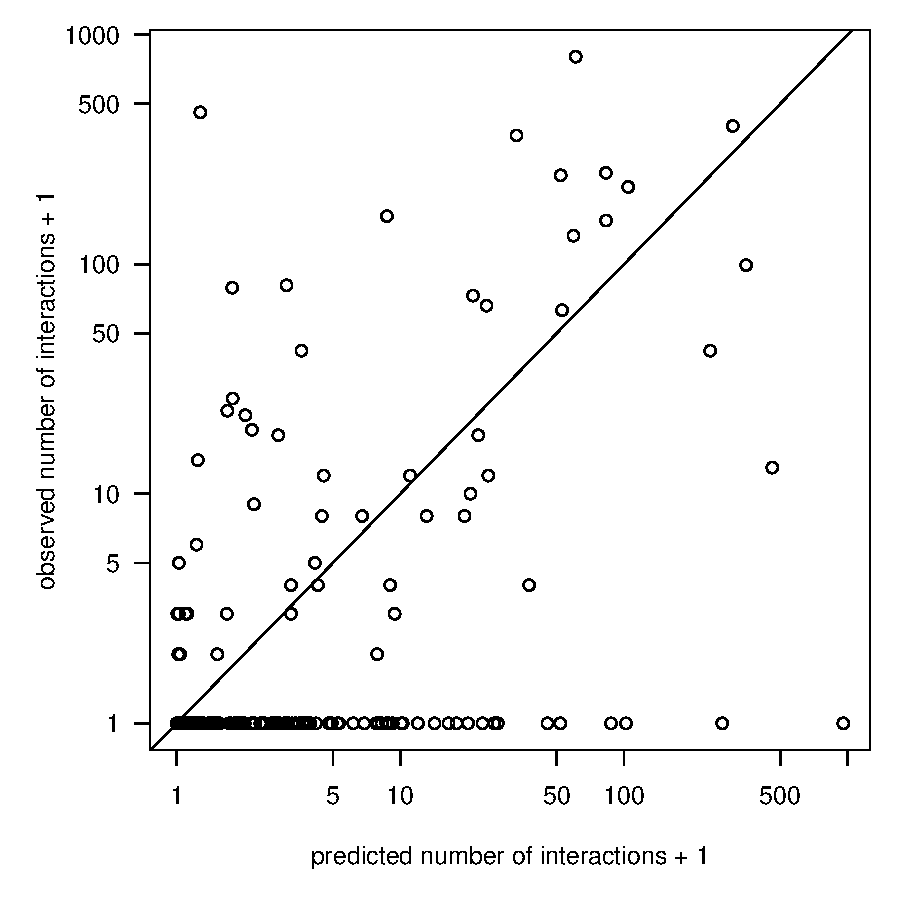
\includegraphics[width=0.5\textwidth]{figure/predict_tapnet_web2_plot-1} 

}



\end{knitrout}
Finally, we can compute the multinomial log-likelihood of the data, given the prediction:
\begin{knitrout}\small
\definecolor{shadecolor}{rgb}{0.969, 0.969, 0.969}\color{fgcolor}\begin{kframe}
\begin{alltt}
\hlkwd{dmultinom}\hlstd{(}\hlkwd{as.vector}\hlstd{(tapnet_web2}\hlopt{$}\hlstd{networks[[}\hlnum{1}\hlstd{]]}\hlopt{$}\hlstd{web),} \hlkwc{prob}\hlstd{=}\hlkwd{as.vector}\hlstd{(preds2.tapnet),}
          \hlkwc{size}\hlstd{=}\hlkwd{sum}\hlstd{(tapnet_web2}\hlopt{$}\hlstd{networks[[}\hlnum{1}\hlstd{]]}\hlopt{$}\hlstd{web),} \hlkwc{log}\hlstd{=T)}
\end{alltt}
\begin{verbatim}
## [1] -9214.783
\end{verbatim}
\end{kframe}
\end{knitrout}


\section{Using multiple networks}
In the tapnet approach, we can also fit several networks simultaneously, and use the resulting fit for prediction. For example, we can fit tapnet to the networks from shrub and cattle, and predict to (1 =) forest:
\begin{knitrout}\small
\definecolor{shadecolor}{rgb}{0.969, 0.969, 0.969}\color{fgcolor}\begin{kframe}
\begin{alltt}
\hlkwd{data}\hlstd{(Tinoco)}
\hlstd{tap} \hlkwb{<-} \hlkwd{make_tapnet}\hlstd{(}\hlkwc{tree_low} \hlstd{= plant_tree,} \hlkwc{tree_high} \hlstd{= humm_tree,} \hlkwc{networks} \hlstd{= networks[}\hlnum{2}\hlopt{:}\hlnum{3}\hlstd{],}
                   \hlkwc{traits_low} \hlstd{= plant_traits,} \hlkwc{traits_high} \hlstd{= humm_traits,}
                   \hlkwc{abun_low} \hlstd{= plant_abun[}\hlnum{2}\hlopt{:}\hlnum{3}\hlstd{],} \hlkwc{abun_high}\hlstd{=humm_abun[}\hlnum{2}\hlopt{:}\hlnum{3}\hlstd{] ,} \hlkwc{npems_lat} \hlstd{=} \hlnum{4}\hlstd{)}
\hlstd{fit} \hlkwb{<-} \hlkwd{fit_tapnet}\hlstd{(tap)} \hlcom{# uses two networks for fitting!}
\hlkwd{gof_tapnet}\hlstd{(fit)}
\end{alltt}
\begin{verbatim}
## $bc_sim_web
## [1] 0.3788003 0.4667962
## 
## $cor_web
## [1] 0.3992802 0.5672018
## 
## $net_indices
## $net_indices[[1]]
##           Index   Observed       Mean     Median       q2.5      q97.5
## 1   connectance  0.2324561  0.7164868  0.7107843  0.6578947  0.7914439
## 2          NODF 43.5864979 81.1276132 81.5320299 73.2460589 86.9142656
## 3 weighted NODF 30.7805907 64.0236824 64.3139011 56.9753183 69.5455754
## 4            H2  0.5022179  0.1207073  0.1206267  0.1110184  0.1307422
## 
## $net_indices[[2]]
##           Index   Observed       Mean     Median       q2.5      q97.5
## 1   connectance  0.3040936  0.6559816  0.6491228  0.6081871  0.7291941
## 2          NODF 56.5180793 81.0418944 81.3004335 73.9846550 87.0980051
## 3 weighted NODF 38.3391890 63.4218334 63.5538500 56.7025985 69.5373901
## 4            H2  0.3713669  0.1161382  0.1163632  0.1020925  0.1303586
\end{verbatim}
\begin{alltt}
\hlcom{# predict to omitted forest network:}
\hlstd{pred1} \hlkwb{<-} \hlkwd{predict_tapnet}\hlstd{(fit,} \hlkwc{abuns}\hlstd{=}\hlkwd{list}\hlstd{(}\hlstr{"low"}\hlstd{=plant_abun[[}\hlnum{1}\hlstd{]],} \hlstr{"high"}\hlstd{=humm_abun[[}\hlnum{1}\hlstd{]] ))}

\hlkwd{cor}\hlstd{(}\hlkwd{as.vector}\hlstd{(pred1}\hlopt{*}\hlkwd{sum}\hlstd{(networks[[}\hlnum{1}\hlstd{]])),} \hlkwd{as.vector}\hlstd{(networks[[}\hlnum{1}\hlstd{]]))}
\end{alltt}
\begin{verbatim}
## [1] 0.1188132
\end{verbatim}
\end{kframe}
\end{knitrout}
And we can do the same for the other two networks (first to 2 = shrubs, then to 3 = cattle):
\begin{knitrout}\small
\definecolor{shadecolor}{rgb}{0.969, 0.969, 0.969}\color{fgcolor}\begin{kframe}
\begin{verbatim}
## [1] 0.1732161
\end{verbatim}
\end{kframe}
\end{knitrout}
\begin{knitrout}\small
\definecolor{shadecolor}{rgb}{0.969, 0.969, 0.969}\color{fgcolor}\begin{kframe}
\begin{verbatim}
## [1] 0.4418444
\end{verbatim}
\end{kframe}
\end{knitrout}
If we compare this single-network predictions (see towards the end of this document), we notice a variable effect on performance: more is not necessarily better. This will probably depend on the similarity of the habitats and hence interacting species.



\section{Prediction baseline: use only abundances in the new web}
As a baseline, we compute the information contained in the abundances. If the hummingbirds had no preferences, but only interacted strictly with probability proportional to abundance, then abundant hummingbird species would interact with high probability with abundant plant species, but with low probability with rare plant species.
\begin{knitrout}\small
\definecolor{shadecolor}{rgb}{0.969, 0.969, 0.969}\color{fgcolor}\begin{kframe}
\begin{alltt}
\hlstd{preds2.abunonly} \hlkwb{<-} \hlstd{(tapnet_web2}\hlopt{$}\hlstd{networks[[}\hlnum{1}\hlstd{]]}\hlopt{$}\hlstd{abuns}\hlopt{$}\hlstd{low} \hlopt{/}
    \hlkwd{sum}\hlstd{(tapnet_web2}\hlopt{$}\hlstd{networks[[}\hlnum{1}\hlstd{]]}\hlopt{$}\hlstd{abuns}\hlopt{$}\hlstd{low))} \hlopt \hlkwd{t}\hlstd{(tapnet_web2}\hlopt{$}\hlstd{networks[[}\hlnum{1}\hlstd{]]}\hlopt{$}\hlstd{abuns}\hlopt{$}\hlstd{high} \hlopt{/}
    \hlkwd{sum}\hlstd{(tapnet_web2}\hlopt{$}\hlstd{networks[[}\hlnum{1}\hlstd{]]}\hlopt{$}\hlstd{abuns}\hlopt{$}\hlstd{high))} \hlopt{*} \hlkwd{sum}\hlstd{(tapnet_web2}\hlopt{$}\hlstd{networks[[}\hlnum{1}\hlstd{]]}\hlopt{$}\hlstd{web)}
\hlkwd{cor}\hlstd{(}\hlkwd{as.vector}\hlstd{(preds2.abunonly),} \hlkwd{as.vector}\hlstd{(tapnet_web2}\hlopt{$}\hlstd{networks[[}\hlnum{1}\hlstd{]]}\hlopt{$}\hlstd{web))}
\end{alltt}
\begin{verbatim}
## [1] 0.09473036
\end{verbatim}
\end{kframe}
\end{knitrout}
\begin{knitrout}\small
\definecolor{shadecolor}{rgb}{0.969, 0.969, 0.969}\color{fgcolor}\begin{kframe}
\begin{alltt}
\hlkwd{par}\hlstd{(}\hlkwc{mar}\hlstd{=}\hlkwd{c}\hlstd{(}\hlnum{5}\hlstd{,}\hlnum{5}\hlstd{,}\hlnum{1}\hlstd{,}\hlnum{1}\hlstd{))}
\hlkwd{plot}\hlstd{(preds2.abunonly} \hlopt{+} \hlnum{1}\hlstd{, tapnet_web2}\hlopt{$}\hlstd{networks[[}\hlnum{1}\hlstd{]]}\hlopt{$}\hlstd{web} \hlopt{+} \hlnum{1}\hlstd{,} \hlkwc{log}\hlstd{=}\hlstr{"xy"}\hlstd{,} \hlkwc{las}\hlstd{=}\hlnum{1}\hlstd{,}
  \hlkwc{xlab}\hlstd{=}\hlstr{"predicted number of interactions + 1"}\hlstd{,} \hlkwc{ylab}\hlstd{=}\hlstr{"observed number of interactions + 1"}\hlstd{)}
\hlkwd{abline}\hlstd{(}\hlnum{0}\hlstd{,}\hlnum{1}\hlstd{)}
\end{alltt}
\end{kframe}

{\centering 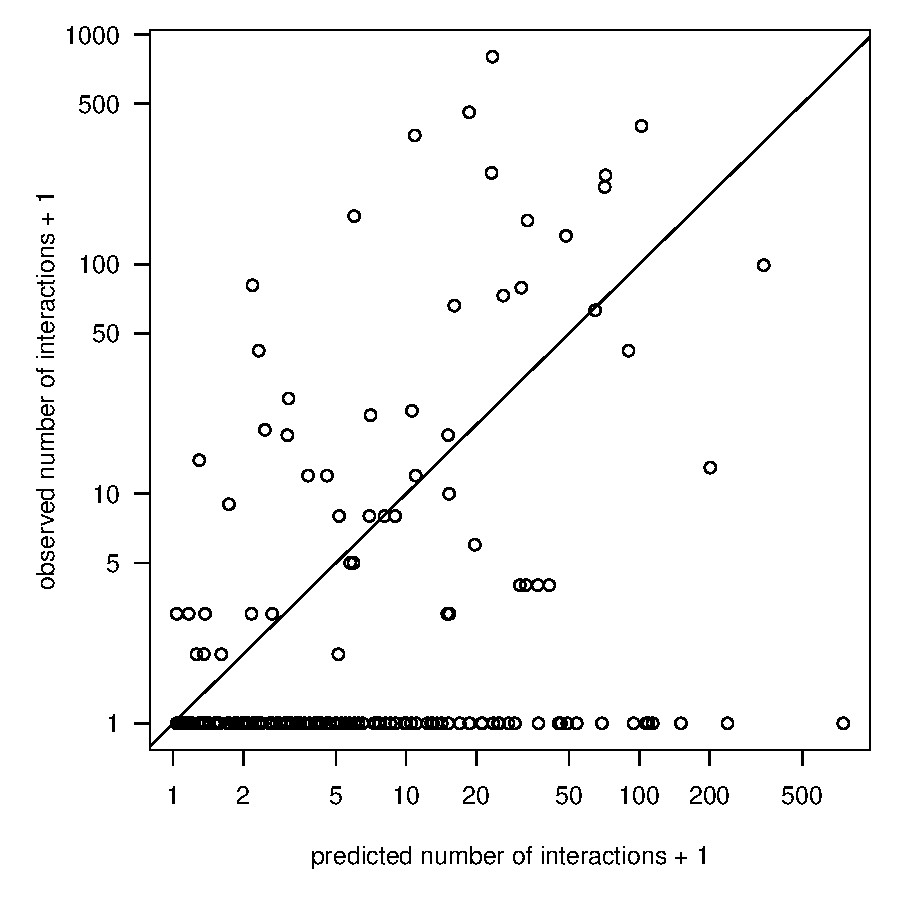
\includegraphics[width=0.5\textwidth]{figure/abunonly_plot-1} 

}



\end{knitrout}
And the log-likelihood:
\begin{knitrout}\small
\definecolor{shadecolor}{rgb}{0.969, 0.969, 0.969}\color{fgcolor}\begin{kframe}
\begin{alltt}
\hlkwd{dmultinom}\hlstd{(}\hlkwd{as.vector}\hlstd{(tapnet_web2}\hlopt{$}\hlstd{networks[[}\hlnum{1}\hlstd{]]}\hlopt{$}\hlstd{web),} \hlkwc{prob}\hlstd{=}\hlkwd{as.vector}\hlstd{(preds2.abunonly),}
          \hlkwc{size}\hlstd{=}\hlkwd{sum}\hlstd{(tapnet_web2}\hlopt{$}\hlstd{networks[[}\hlnum{1}\hlstd{]]}\hlopt{$}\hlstd{web),} \hlkwc{log}\hlstd{=T)}
\end{alltt}
\begin{verbatim}
## [1] -9202.007
\end{verbatim}
\end{kframe}
\end{knitrout}
This means, our tapnet model is superior in prediction to the abundance-only model, indicating that the (latent and observed) traits do carry some information on the interactions. Note, however, that the prediction quality of the abundance-only is very low.



\section{Preparing tapnet data as data.frame for statistical models}
To prepare the data for a statistical model, we provide the function \code{tapnet2df}:
\begin{knitrout}\small
\definecolor{shadecolor}{rgb}{0.969, 0.969, 0.969}\color{fgcolor}\begin{kframe}
\begin{alltt}
\hlstd{web1.df} \hlkwb{<-} \hlkwd{tapnet2df}\hlstd{(tapnet_web1)}
\hlstd{web2.df} \hlkwb{<-} \hlkwd{tapnet2df}\hlstd{(tapnet_web2)}
\hlkwd{head}\hlstd{(web1.df)}
\end{alltt}
\begin{verbatim}
##         IDhigher                IDlower interactions     pemLV_1     pemLV_2
## 1 Coeligena iris Alloplectus peruvianum           13  0.19958316 -0.01721758
## 2 Coeligena iris    Macleania rupestris           22  0.06143519  0.01314354
## 3 Coeligena iris   Myrcianthes fragrans            0 -0.17608854  0.22809965
## 4 Coeligena iris           Salvia hirta            4  0.21167754 -0.01945177
## 5 Coeligena iris  Cavendishia bracteata            0  0.06143519  0.01314354
## 6 Coeligena iris      Mutisia lehmannii            6  0.20823846 -0.02230535
##        pemLV_3      pemLV_7   pemHV_1    pemHV_3    pemHV_6   pemHV_8     abunL
## 1  0.298458999  0.110246748 0.3026318 0.09104722 -0.2849888 0.5647174  3.428571
## 2  0.014975823  0.006401991 0.3026318 0.09104722 -0.2849888 0.5647174 38.529412
## 3 -0.006808424 -0.005932541 0.3026318 0.09104722 -0.2849888 0.5647174 69.500000
## 4  0.346816571  0.323487833 0.3026318 0.09104722 -0.2849888 0.5647174 10.783505
## 5  0.014975823  0.006401991 0.3026318 0.09104722 -0.2849888 0.5647174 26.111111
## 6 -0.310376666  0.013295514 0.3026318 0.09104722 -0.2849888 0.5647174  2.740741
##      abunH traitLCorolla_length_mm traitHBill_length_mean_mm
## 1 3.950695                    48.1                      28.1
## 2 3.950695                    16.5                      28.1
## 3 3.950695                     1.3                      28.1
## 4 3.950695                    22.9                      28.1
## 5 3.950695                    24.5                      28.1
## 6 3.950695                    29.3                      28.1
\end{verbatim}
\end{kframe}
\end{knitrout}
These data.frames contain all the information coded in the tapnet object, but no matches of traits.



\section{Prediction using GAM of phylogeny, traits and trait matching}
To apply the approach of Brousseau et al. (2018) to our quantitative network, we use a negative binomial GAM. It uses, as predictors, the first two PEMs of each group, plus the observed traits, plus the squared trait difference, plus the abundances.

We augment the data.frames from the previous section by the trait-matching variables (in this case only one pair: bill and corolla length):
\begin{knitrout}\small
\definecolor{shadecolor}{rgb}{0.969, 0.969, 0.969}\color{fgcolor}\begin{kframe}
\begin{alltt}
\hlstd{web1.df.extended} \hlkwb{<-} \hlkwd{cbind.data.frame}\hlstd{(web1.df,} \hlstr{"match"}\hlstd{=(web1.df}\hlopt{$}\hlstd{traitHBill_length_mean_mm} \hlopt{-}
                                                  \hlstd{web1.df}\hlopt{$}\hlstd{traitLCorolla_length_mm)}\hlopt{^}\hlnum{2} \hlstd{)}
\hlstd{web2.df.extended} \hlkwb{<-} \hlkwd{cbind.data.frame}\hlstd{(web2.df,} \hlstr{"match"}\hlstd{=(web2.df}\hlopt{$}\hlstd{traitHBill_length_mean_mm} \hlopt{-}
                                                  \hlstd{web2.df}\hlopt{$}\hlstd{traitLCorolla_length_mm)}\hlopt{^}\hlnum{2} \hlstd{)}
\end{alltt}
\end{kframe}
\end{knitrout}
Now we can fit the model. Note that we believe this approach to be statistically incorrect, as it assumes that the observed interactions are independent, when (clearly?) they are not. Each bird selects a flower based on what is on offer; thus, a decision to visit one flower implies \emph{not} visiting another, creating a negative dependence. Anyway.
\begin{knitrout}\small
\definecolor{shadecolor}{rgb}{0.969, 0.969, 0.969}\color{fgcolor}\begin{kframe}
\begin{alltt}
\hlkwd{library}\hlstd{(mgcv)}
\hlstd{gam2} \hlkwb{<-} \hlkwd{gam}\hlstd{(interactions} \hlopt{~} \hlkwd{s}\hlstd{(pemLV_1, pemHV_1,} \hlkwc{bs}\hlstd{=}\hlstr{"ts"}\hlstd{,} \hlkwc{k}\hlstd{=}\hlnum{24}\hlstd{)} \hlopt{+}\hlkwd{s}\hlstd{(pemLV_2, pemHV_3,} \hlkwc{bs}\hlstd{=}\hlstr{"ts"}\hlstd{,}
           \hlkwc{k}\hlstd{=}\hlnum{24}\hlstd{)} \hlopt{+} \hlkwd{s}\hlstd{(traitLCorolla_length_mm,} \hlkwc{k}\hlstd{=}\hlnum{3}\hlstd{)} \hlopt{+} \hlkwd{s}\hlstd{(traitHBill_length_mean_mm,} \hlkwc{k}\hlstd{=}\hlnum{3}\hlstd{)} \hlopt{+}
           \hlkwd{s}\hlstd{(match,} \hlkwc{k}\hlstd{=}\hlnum{3}\hlstd{)} \hlopt{+} \hlkwd{s}\hlstd{(abunL,} \hlkwc{k}\hlstd{=}\hlnum{3}\hlstd{)} \hlopt{+} \hlkwd{s}\hlstd{(abunH,} \hlkwc{k}\hlstd{=}\hlnum{3}\hlstd{),} \hlkwc{data}\hlstd{=web1.df.extended,} \hlkwc{family}\hlstd{=nb,}
           \hlkwc{gamma}\hlstd{=}\hlnum{1.4}\hlstd{)}
\hlkwd{summary}\hlstd{(gam2)}
\end{alltt}
\begin{verbatim}
## 
## Family: Negative Binomial(0.171) 
## Link function: log 
## 
## Formula:
## interactions ~ s(pemLV_1, pemHV_1, bs = "ts", k = 24) + s(pemLV_2, 
##     pemHV_3, bs = "ts", k = 24) + s(traitLCorolla_length_mm, 
##     k = 3) + s(traitHBill_length_mean_mm, k = 3) + s(match, k = 3) + 
##     s(abunL, k = 3) + s(abunH, k = 3)
## 
## Parametric coefficients:
##             Estimate Std. Error z value Pr(>|z|)    
## (Intercept)   -5.969      1.703  -3.505 0.000456 ***
## ---
## Signif. codes:  0 '***' 0.001 '**' 0.01 '*' 0.05 '.' 0.1 ' ' 1
## 
## Approximate significance of smooth terms:
##                                    edf Ref.df Chi.sq  p-value    
## s(pemLV_1,pemHV_1)           1.480e+00 23.000 14.647 7.86e-05 ***
## s(pemLV_2,pemHV_3)           1.724e-05 23.000  0.000 0.291704    
## s(traitLCorolla_length_mm)   1.772e+00  1.929 10.635 0.002754 ** 
## s(traitHBill_length_mean_mm) 1.000e+00  1.000  0.442 0.506187    
## s(match)                     1.000e+00  1.000 18.939 1.38e-05 ***
## s(abunL)                     1.917e+00  1.993 14.489 0.001103 ** 
## s(abunH)                     1.000e+00  1.000 12.618 0.000382 ***
## ---
## Signif. codes:  0 '***' 0.001 '**' 0.01 '*' 0.05 '.' 0.1 ' ' 1
## 
## R-sq.(adj) =     -5   Deviance explained = 49.3%
## -REML =    203  Scale est. = 1         n = 160
\end{verbatim}
\begin{alltt}
\hlstd{preds2.gam} \hlkwb{<-} \hlkwd{predict}\hlstd{(gam2,} \hlkwc{newdata}\hlstd{=web2.df.extended)}
\hlkwd{cor}\hlstd{(}\hlkwd{exp}\hlstd{(preds2.gam), web2.df}\hlopt{$}\hlstd{interactions)}
\end{alltt}
\begin{verbatim}
## [1] -0.01210051
\end{verbatim}
\end{kframe}
\end{knitrout}
Here, the contributions of the different predictors can easily be discerned. Abundances and trait-matching are important, but phylogenetics are (apparently) not. Note that in this case corolla length and trait matching are high ($r=0.84$) correlated, representing the same information. That could be avoided by standardising the trait values before fitting the model. However, in that case we lose the direct interpretation of 0 indicating the same length of corolla and bill.

Again, we can plot the result:
\begin{knitrout}\small
\definecolor{shadecolor}{rgb}{0.969, 0.969, 0.969}\color{fgcolor}\begin{kframe}
\begin{alltt}
\hlkwd{par}\hlstd{(}\hlkwc{mar}\hlstd{=}\hlkwd{c}\hlstd{(}\hlnum{5}\hlstd{,}\hlnum{5}\hlstd{,}\hlnum{1}\hlstd{,}\hlnum{1}\hlstd{))}
\hlkwd{plot}\hlstd{(}\hlkwd{exp}\hlstd{(preds2.gam)} \hlopt{+}\hlnum{1} \hlstd{, web2.df}\hlopt{$}\hlstd{interactions} \hlopt{+} \hlnum{1}\hlstd{,} \hlkwc{log}\hlstd{=}\hlstr{"xy"}\hlstd{,} \hlkwc{las}\hlstd{=}\hlnum{1}\hlstd{,} \hlkwc{xlab}\hlstd{=}\hlstr{"predicted 
     number of interactions + 1"}\hlstd{,} \hlkwc{ylab}\hlstd{=}\hlstr{"observed number of interactions + 1"}\hlstd{)}
\hlkwd{abline}\hlstd{(}\hlnum{0}\hlstd{,}\hlnum{1}\hlstd{)}
\end{alltt}
\end{kframe}

{\centering 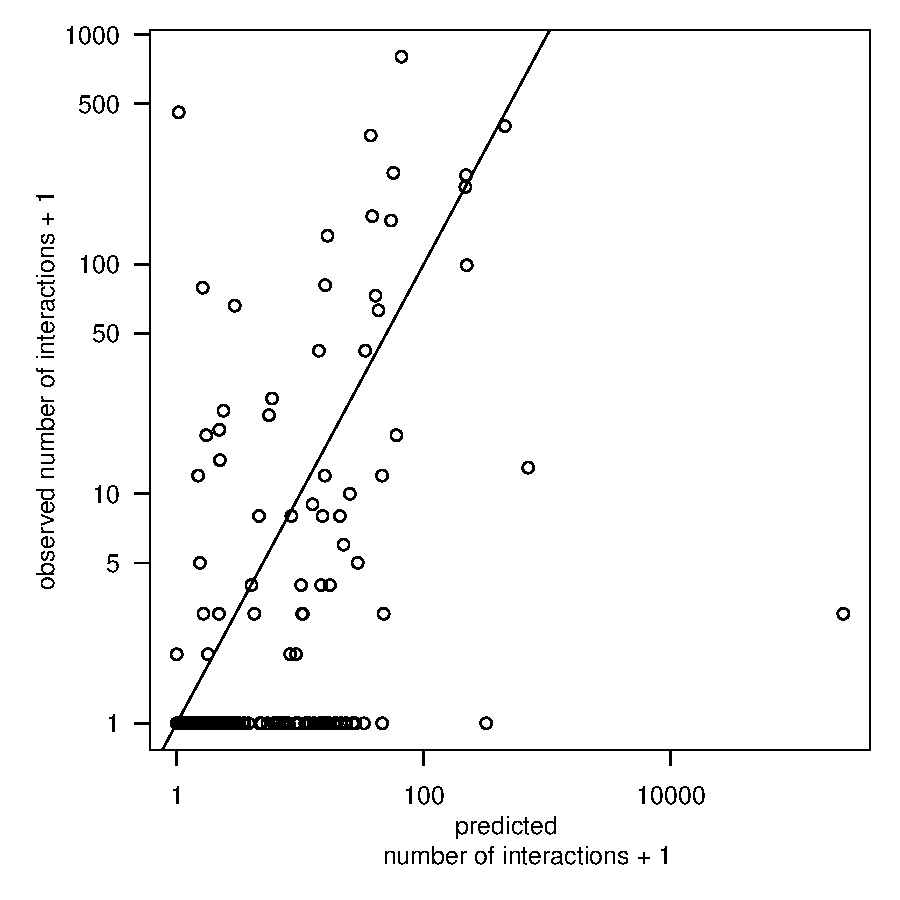
\includegraphics[width=0.5\textwidth]{figure/predict_2_gam_plot-1} 

}



\end{knitrout}
This prediction contains no information on the observed interactions.

And the log-likelihood:
\begin{knitrout}\small
\definecolor{shadecolor}{rgb}{0.969, 0.969, 0.969}\color{fgcolor}\begin{kframe}
\begin{alltt}
\hlkwd{dmultinom}\hlstd{(}\hlkwd{as.vector}\hlstd{(tapnet_web2}\hlopt{$}\hlstd{networks[[}\hlnum{1}\hlstd{]]}\hlopt{$}\hlstd{web),} \hlkwc{prob}\hlstd{=}\hlkwd{exp}\hlstd{(preds2.gam)} \hlopt{/}
            \hlkwd{sum}\hlstd{(}\hlkwd{exp}\hlstd{(preds2.gam)),} \hlkwc{size}\hlstd{=}\hlkwd{sum}\hlstd{(tapnet_web2}\hlopt{$}\hlstd{networks[[}\hlnum{1}\hlstd{]]}\hlopt{$}\hlstd{web),} \hlkwc{log}\hlstd{=T)}
\end{alltt}
\begin{verbatim}
## [1] -144756.9
\end{verbatim}
\end{kframe}
\end{knitrout}
So these values are abysmally poor.


\section{Prediction using randomForest with phylogeny, traits and trait matching}
We can use the same data with a different algorithm, in this case randomForest (as implemented in ranger). It provides an assessment of which predictors are important to the fit:
\begin{knitrout}\small
\definecolor{shadecolor}{rgb}{0.969, 0.969, 0.969}\color{fgcolor}\begin{kframe}
\begin{alltt}
\hlkwd{library}\hlstd{(ranger)}
\hlstd{rf2} \hlkwb{<-} \hlkwd{ranger}\hlstd{(interactions} \hlopt{~} \hlstd{.,} \hlkwc{data}\hlstd{=web1.df.extended[,} \hlopt{-}\hlkwd{c}\hlstd{(}\hlnum{1}\hlstd{,} \hlnum{2}\hlstd{)],} \hlkwc{importance}\hlstd{=}\hlstr{"impurity"}\hlstd{)}
\hlstd{rf2}
\end{alltt}
\begin{verbatim}
## Ranger result
## 
## Call:
##  ranger(interactions ~ ., data = web1.df.extended[, -c(1, 2)],      importance = "impurity") 
## 
## Type:                             Regression 
## Number of trees:                  500 
## Sample size:                      160 
## Number of independent variables:  13 
## Mtry:                             3 
## Target node size:                 5 
## Variable importance mode:         impurity 
## Splitrule:                        variance 
## OOB prediction error (MSE):       599.1792 
## R squared (OOB):                  0.0733405
\end{verbatim}
\begin{alltt}
\hlkwd{sort}\hlstd{(}\hlkwd{importance}\hlstd{(rf2),} \hlkwc{decreasing}\hlstd{=T)}
\end{alltt}
\begin{verbatim}
##                     abunL                     match   traitLCorolla_length_mm 
##                 12558.832                 12170.222                  9190.177 
##                   pemLV_2                   pemHV_3                     abunH 
##                  7706.507                  6818.601                  6332.438 
## traitHBill_length_mean_mm                   pemHV_1                   pemLV_3 
##                  5743.067                  4890.467                  4836.141 
##                   pemLV_1                   pemLV_7                   pemHV_6 
##                  4729.878                  4617.740                  1195.166 
##                   pemHV_8 
##                  1085.502
\end{verbatim}
\end{kframe}
\end{knitrout}

\begin{knitrout}\small
\definecolor{shadecolor}{rgb}{0.969, 0.969, 0.969}\color{fgcolor}\begin{kframe}
\begin{alltt}
\hlstd{preds2.ranger} \hlkwb{<-} \hlkwd{predict}\hlstd{(rf2,} \hlkwc{data}\hlstd{=web2.df.extended)}\hlopt{$}\hlstd{predictions}
\hlkwd{cor}\hlstd{(preds2.ranger, web2.df}\hlopt{$}\hlstd{interactions)}
\end{alltt}
\begin{verbatim}
## [1] 0.2219289
\end{verbatim}
\begin{alltt}
\hlkwd{par}\hlstd{(}\hlkwc{mar}\hlstd{=}\hlkwd{c}\hlstd{(}\hlnum{5}\hlstd{,}\hlnum{5}\hlstd{,}\hlnum{1}\hlstd{,}\hlnum{1}\hlstd{))}
\hlkwd{plot}\hlstd{(preds2.ranger} \hlopt{+}\hlnum{1} \hlstd{, web2.df}\hlopt{$}\hlstd{interactions} \hlopt{+} \hlnum{1}\hlstd{,} \hlkwc{log}\hlstd{=}\hlstr{"xy"}\hlstd{,} \hlkwc{las}\hlstd{=}\hlnum{1}\hlstd{,} \hlkwc{xlab}\hlstd{=}\hlstr{"predicted number 
     of interactions + 1"}\hlstd{,} \hlkwc{ylab}\hlstd{=}\hlstr{"observed number of interactions + 1"}\hlstd{)}
\hlkwd{abline}\hlstd{(}\hlnum{0}\hlstd{,}\hlnum{1}\hlstd{)}
\end{alltt}
\end{kframe}

{\centering 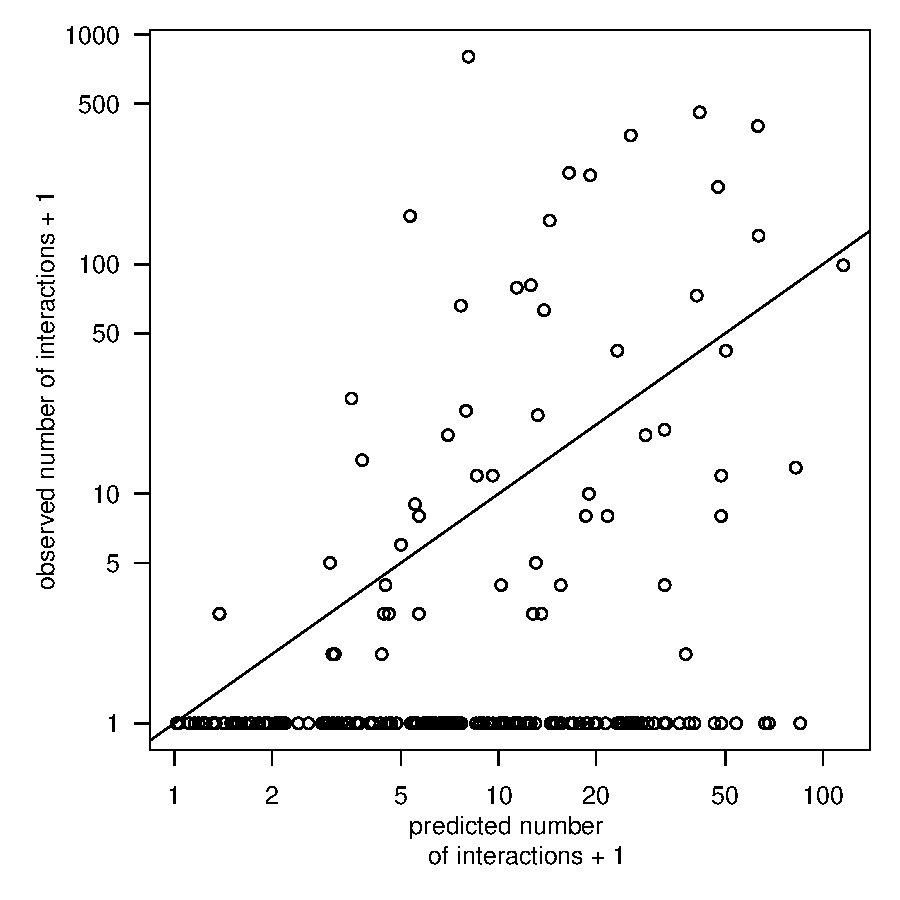
\includegraphics[width=0.5\textwidth]{figure/plot_ranger_predictions_web2-1} 

}



\end{knitrout}

And the log-likelihood:
\begin{knitrout}\small
\definecolor{shadecolor}{rgb}{0.969, 0.969, 0.969}\color{fgcolor}\begin{kframe}
\begin{alltt}
\hlkwd{dmultinom}\hlstd{(}\hlkwd{as.vector}\hlstd{(tapnet_web2}\hlopt{$}\hlstd{networks[[}\hlnum{1}\hlstd{]]}\hlopt{$}\hlstd{web),} \hlkwc{prob}\hlstd{=preds2.ranger}\hlopt{/}\hlkwd{sum}\hlstd{(preds2.ranger),}
          \hlkwc{size}\hlstd{=}\hlkwd{sum}\hlstd{(tapnet_web2}\hlopt{$}\hlstd{networks[[}\hlnum{1}\hlstd{]]}\hlopt{$}\hlstd{web),} \hlkwc{log}\hlstd{=T)}
\end{alltt}
\begin{verbatim}
## [1] -11929.07
\end{verbatim}
\end{kframe}
\end{knitrout}

This model is better than the abundance-only, GAM -- and tapnet.



\section{Cross-validation for all approaches}
Here we only present the code and results for the cross-validation, where the model it fit to one web and predicts to the other two, for all three combinations. We use the same settings and data preparation as in the sections above.

\subsection{Using tapnet}
\begin{knitrout}\small
\definecolor{shadecolor}{rgb}{0.969, 0.969, 0.969}\color{fgcolor}\begin{kframe}
\begin{alltt}
\hlstd{tapnet_web1} \hlkwb{<-} \hlkwd{make_tapnet}\hlstd{(}\hlkwc{tree_low}\hlstd{=plant_tree,} \hlkwc{tree_high}\hlstd{=humm_tree,} \hlkwc{networks}\hlstd{=networks[}\hlnum{1}\hlstd{],}
                           \hlkwc{traits_low}\hlstd{=plant_traits,} \hlkwc{traits_high}\hlstd{=humm_traits,}
                           \hlkwc{abun_low}\hlstd{=plant_abun[}\hlnum{1}\hlstd{],} \hlkwc{abun_high}\hlstd{=humm_abun[}\hlnum{1}\hlstd{],} \hlkwc{npems_lat}\hlstd{=}\hlnum{4}\hlstd{)}
\hlstd{tapnet_web2} \hlkwb{<-} \hlkwd{make_tapnet}\hlstd{(}\hlkwc{tree_low}\hlstd{=plant_tree,} \hlkwc{tree_high}\hlstd{=humm_tree,} \hlkwc{networks}\hlstd{=networks[}\hlnum{2}\hlstd{],}
                           \hlkwc{traits_low}\hlstd{=plant_traits,} \hlkwc{traits_high}\hlstd{=humm_traits,}
                           \hlkwc{abun_low}\hlstd{=plant_abun[}\hlnum{2}\hlstd{],} \hlkwc{abun_high}\hlstd{=humm_abun[}\hlnum{2}\hlstd{],} \hlkwc{npems_lat}\hlstd{=}\hlnum{4}\hlstd{)}
\hlstd{tapnet_web3} \hlkwb{<-} \hlkwd{make_tapnet}\hlstd{(}\hlkwc{tree_low}\hlstd{=plant_tree,} \hlkwc{tree_high}\hlstd{=humm_tree,} \hlkwc{networks}\hlstd{=networks[}\hlnum{3}\hlstd{],}
                           \hlkwc{traits_low}\hlstd{=plant_traits,} \hlkwc{traits_high}\hlstd{=humm_traits,}
                           \hlkwc{abun_low}\hlstd{=plant_abun[}\hlnum{3}\hlstd{],} \hlkwc{abun_high}\hlstd{=humm_abun[}\hlnum{3}\hlstd{],} \hlkwc{npems_lat}\hlstd{=}\hlnum{4}\hlstd{)}
\end{alltt}
\end{kframe}
\end{knitrout}
\begin{knitrout}\small
\definecolor{shadecolor}{rgb}{0.969, 0.969, 0.969}\color{fgcolor}\begin{kframe}
\begin{alltt}
\hlstd{fit_web1} \hlkwb{<-} \hlkwd{fit_tapnet}\hlstd{(}\hlkwc{tapnet} \hlstd{= tapnet_web1,} \hlkwc{method}\hlstd{=}\hlstr{"SANN"}\hlstd{)}
\hlstd{fit_web2} \hlkwb{<-} \hlkwd{fit_tapnet}\hlstd{(}\hlkwc{tapnet} \hlstd{= tapnet_web2,} \hlkwc{method}\hlstd{=}\hlstr{"SANN"}\hlstd{)}
\hlstd{fit_web3} \hlkwb{<-} \hlkwd{fit_tapnet}\hlstd{(}\hlkwc{tapnet} \hlstd{= tapnet_web3,} \hlkwc{method}\hlstd{=}\hlstr{"SANN"}\hlstd{)}
\end{alltt}
\end{kframe}
\end{knitrout}
\begin{knitrout}\small
\definecolor{shadecolor}{rgb}{0.969, 0.969, 0.969}\color{fgcolor}\begin{kframe}
\begin{alltt}
\hlopt{-}\hlkwd{c}\hlstd{(fit_web1}\hlopt{$}\hlstd{opt}\hlopt{$}\hlstd{value, fit_web2}\hlopt{$}\hlstd{opt}\hlopt{$}\hlstd{value, fit_web3}\hlopt{$}\hlstd{opt}\hlopt{$}\hlstd{value)}
\end{alltt}
\begin{verbatim}
## [1] -1726.225 -4331.951 -1901.977
\end{verbatim}
\end{kframe}
\end{knitrout}

\begin{knitrout}\small
\definecolor{shadecolor}{rgb}{0.969, 0.969, 0.969}\color{fgcolor}\begin{kframe}
\begin{alltt}
\hlstd{preds2.tapnet1} \hlkwb{<-} \hlkwd{predict_tapnet}\hlstd{(}\hlkwc{fit}\hlstd{=fit_web1,} \hlkwc{abuns}\hlstd{=tapnet_web2}\hlopt{$}\hlstd{networks[[}\hlnum{1}\hlstd{]]}\hlopt{$}\hlstd{abuns)}
\hlstd{preds3.tapnet1} \hlkwb{<-} \hlkwd{predict_tapnet}\hlstd{(}\hlkwc{fit}\hlstd{=fit_web1,} \hlkwc{abuns}\hlstd{=tapnet_web3}\hlopt{$}\hlstd{networks[[}\hlnum{1}\hlstd{]]}\hlopt{$}\hlstd{abuns)}
\hlstd{preds1.tapnet2} \hlkwb{<-} \hlkwd{predict_tapnet}\hlstd{(}\hlkwc{fit}\hlstd{=fit_web2,} \hlkwc{abuns}\hlstd{=tapnet_web1}\hlopt{$}\hlstd{networks[[}\hlnum{1}\hlstd{]]}\hlopt{$}\hlstd{abuns)}
\hlstd{preds3.tapnet2} \hlkwb{<-} \hlkwd{predict_tapnet}\hlstd{(}\hlkwc{fit}\hlstd{=fit_web2,} \hlkwc{abuns}\hlstd{=tapnet_web3}\hlopt{$}\hlstd{networks[[}\hlnum{1}\hlstd{]]}\hlopt{$}\hlstd{abuns)}
\hlstd{preds1.tapnet3} \hlkwb{<-} \hlkwd{predict_tapnet}\hlstd{(}\hlkwc{fit}\hlstd{=fit_web3,} \hlkwc{abuns}\hlstd{=tapnet_web1}\hlopt{$}\hlstd{networks[[}\hlnum{1}\hlstd{]]}\hlopt{$}\hlstd{abuns)}
\hlstd{preds2.tapnet3} \hlkwb{<-} \hlkwd{predict_tapnet}\hlstd{(}\hlkwc{fit}\hlstd{=fit_web3,} \hlkwc{abuns}\hlstd{=tapnet_web2}\hlopt{$}\hlstd{networks[[}\hlnum{1}\hlstd{]]}\hlopt{$}\hlstd{abuns)}
\end{alltt}
\end{kframe}
\end{knitrout}
%#predList <- list(preds2.tapnet1, preds3.tapnet1, preds1.tapnet2, preds3.tapnet2, preds1.tapnet2, preds2.tapnet2)
\begin{knitrout}\small
\definecolor{shadecolor}{rgb}{0.969, 0.969, 0.969}\color{fgcolor}\begin{kframe}
\begin{alltt}
\hlstd{cors.tapnet} \hlkwb{<-} \hlkwd{c}\hlstd{(}
  \hlkwd{cor}\hlstd{(}\hlkwd{as.vector}\hlstd{(preds2.tapnet1),} \hlkwd{as.vector}\hlstd{(tapnet_web2}\hlopt{$}\hlstd{networks[[}\hlnum{1}\hlstd{]]}\hlopt{$}\hlstd{web)),}
  \hlkwd{cor}\hlstd{(}\hlkwd{as.vector}\hlstd{(preds3.tapnet1),} \hlkwd{as.vector}\hlstd{(tapnet_web3}\hlopt{$}\hlstd{networks[[}\hlnum{1}\hlstd{]]}\hlopt{$}\hlstd{web)),}
  \hlkwd{cor}\hlstd{(}\hlkwd{as.vector}\hlstd{(preds1.tapnet2),} \hlkwd{as.vector}\hlstd{(tapnet_web1}\hlopt{$}\hlstd{networks[[}\hlnum{1}\hlstd{]]}\hlopt{$}\hlstd{web)),}
  \hlkwd{cor}\hlstd{(}\hlkwd{as.vector}\hlstd{(preds3.tapnet2),} \hlkwd{as.vector}\hlstd{(tapnet_web3}\hlopt{$}\hlstd{networks[[}\hlnum{1}\hlstd{]]}\hlopt{$}\hlstd{web)),}
  \hlkwd{cor}\hlstd{(}\hlkwd{as.vector}\hlstd{(preds1.tapnet3),} \hlkwd{as.vector}\hlstd{(tapnet_web1}\hlopt{$}\hlstd{networks[[}\hlnum{1}\hlstd{]]}\hlopt{$}\hlstd{web)),}
  \hlkwd{cor}\hlstd{(}\hlkwd{as.vector}\hlstd{(preds2.tapnet3),} \hlkwd{as.vector}\hlstd{(tapnet_web2}\hlopt{$}\hlstd{networks[[}\hlnum{1}\hlstd{]]}\hlopt{$}\hlstd{web))}
\hlstd{)}
\hlstd{cors.tapnet}
\end{alltt}
\begin{verbatim}
## [1] 0.13508949 0.52398437 0.10842538 0.47967584 0.02909331 0.11391497
\end{verbatim}
\end{kframe}
\end{knitrout}
\begin{knitrout}\small
\definecolor{shadecolor}{rgb}{0.969, 0.969, 0.969}\color{fgcolor}\begin{kframe}
\begin{alltt}
\hlstd{ellCV.tapnet} \hlkwb{<-} \hlkwd{c}\hlstd{(}
  \hlkwd{dmultinom}\hlstd{(}\hlkwd{as.vector}\hlstd{(tapnet_web2}\hlopt{$}\hlstd{networks[[}\hlnum{1}\hlstd{]]}\hlopt{$}\hlstd{web),} \hlkwc{prob}\hlstd{=}\hlkwd{as.vector}\hlstd{(preds2.tapnet1),}
            \hlkwc{size}\hlstd{=}\hlkwd{sum}\hlstd{(tapnet_web2}\hlopt{$}\hlstd{networks[[}\hlnum{1}\hlstd{]]}\hlopt{$}\hlstd{web),} \hlkwc{log}\hlstd{=T),}
  \hlkwd{dmultinom}\hlstd{(}\hlkwd{as.vector}\hlstd{(tapnet_web3}\hlopt{$}\hlstd{networks[[}\hlnum{1}\hlstd{]]}\hlopt{$}\hlstd{web),} \hlkwc{prob}\hlstd{=}\hlkwd{as.vector}\hlstd{(preds3.tapnet1),}
            \hlkwc{size}\hlstd{=}\hlkwd{sum}\hlstd{(tapnet_web3}\hlopt{$}\hlstd{networks[[}\hlnum{1}\hlstd{]]}\hlopt{$}\hlstd{web),} \hlkwc{log}\hlstd{=T),}
  \hlkwd{dmultinom}\hlstd{(}\hlkwd{as.vector}\hlstd{(tapnet_web1}\hlopt{$}\hlstd{networks[[}\hlnum{1}\hlstd{]]}\hlopt{$}\hlstd{web),} \hlkwc{prob}\hlstd{=}\hlkwd{as.vector}\hlstd{(preds1.tapnet2),}
            \hlkwc{size}\hlstd{=}\hlkwd{sum}\hlstd{(tapnet_web1}\hlopt{$}\hlstd{networks[[}\hlnum{1}\hlstd{]]}\hlopt{$}\hlstd{web),} \hlkwc{log}\hlstd{=T),}
  \hlkwd{dmultinom}\hlstd{(}\hlkwd{as.vector}\hlstd{(tapnet_web3}\hlopt{$}\hlstd{networks[[}\hlnum{1}\hlstd{]]}\hlopt{$}\hlstd{web),} \hlkwc{prob}\hlstd{=}\hlkwd{as.vector}\hlstd{(preds3.tapnet2),}
            \hlkwc{size}\hlstd{=}\hlkwd{sum}\hlstd{(tapnet_web3}\hlopt{$}\hlstd{networks[[}\hlnum{1}\hlstd{]]}\hlopt{$}\hlstd{web),} \hlkwc{log}\hlstd{=T),}
  \hlkwd{dmultinom}\hlstd{(}\hlkwd{as.vector}\hlstd{(tapnet_web1}\hlopt{$}\hlstd{networks[[}\hlnum{1}\hlstd{]]}\hlopt{$}\hlstd{web),} \hlkwc{prob}\hlstd{=}\hlkwd{as.vector}\hlstd{(preds1.tapnet3),}
            \hlkwc{size}\hlstd{=}\hlkwd{sum}\hlstd{(tapnet_web1}\hlopt{$}\hlstd{networks[[}\hlnum{1}\hlstd{]]}\hlopt{$}\hlstd{web),} \hlkwc{log}\hlstd{=T),}
  \hlkwd{dmultinom}\hlstd{(}\hlkwd{as.vector}\hlstd{(tapnet_web2}\hlopt{$}\hlstd{networks[[}\hlnum{1}\hlstd{]]}\hlopt{$}\hlstd{web),} \hlkwc{prob}\hlstd{=}\hlkwd{as.vector}\hlstd{(preds2.tapnet3),}
            \hlkwc{size}\hlstd{=}\hlkwd{sum}\hlstd{(tapnet_web2}\hlopt{$}\hlstd{networks[[}\hlnum{1}\hlstd{]]}\hlopt{$}\hlstd{web),} \hlkwc{log}\hlstd{=T)}
\hlstd{)}
\hlstd{ellCV.tapnet}
\end{alltt}
\begin{verbatim}
## [1] -7992.325 -2838.724 -2893.864 -4553.146 -3175.828 -8479.723
\end{verbatim}
\end{kframe}
\end{knitrout}
\subsection{Fit of the baseline, abundance-only model}
\begin{knitrout}\small
\definecolor{shadecolor}{rgb}{0.969, 0.969, 0.969}\color{fgcolor}\begin{kframe}
\begin{alltt}
\hlstd{preds1.abunonly} \hlkwb{<-} \hlstd{(tapnet_web1}\hlopt{$}\hlstd{networks[[}\hlnum{1}\hlstd{]]}\hlopt{$}\hlstd{abuns}\hlopt{$}\hlstd{low} \hlopt{/}
        \hlkwd{sum}\hlstd{(tapnet_web1}\hlopt{$}\hlstd{networks[[}\hlnum{1}\hlstd{]]}\hlopt{$}\hlstd{abuns}\hlopt{$}\hlstd{low))} \hlopt \hlkwd{t}\hlstd{(tapnet_web1}\hlopt{$}\hlstd{networks[[}\hlnum{1}\hlstd{]]}\hlopt{$}\hlstd{abuns}\hlopt{$}\hlstd{high} \hlopt{/}
        \hlkwd{sum}\hlstd{(tapnet_web1}\hlopt{$}\hlstd{networks[[}\hlnum{1}\hlstd{]]}\hlopt{$}\hlstd{abuns}\hlopt{$}\hlstd{high))} \hlopt{/} \hlkwd{sum}\hlstd{(tapnet_web1}\hlopt{$}\hlstd{networks[[}\hlnum{1}\hlstd{]]}\hlopt{$}\hlstd{web)}
\hlstd{preds2.abunonly} \hlkwb{<-} \hlstd{(tapnet_web2}\hlopt{$}\hlstd{networks[[}\hlnum{1}\hlstd{]]}\hlopt{$}\hlstd{abuns}\hlopt{$}\hlstd{low} \hlopt{/}
      \hlkwd{sum}\hlstd{(tapnet_web2}\hlopt{$}\hlstd{networks[[}\hlnum{1}\hlstd{]]}\hlopt{$}\hlstd{abuns}\hlopt{$}\hlstd{low))} \hlopt \hlkwd{t}\hlstd{(tapnet_web2}\hlopt{$}\hlstd{networks[[}\hlnum{1}\hlstd{]]}\hlopt{$}\hlstd{abuns}\hlopt{$}\hlstd{high} \hlopt{/}
      \hlkwd{sum}\hlstd{(tapnet_web2}\hlopt{$}\hlstd{networks[[}\hlnum{1}\hlstd{]]}\hlopt{$}\hlstd{abuns}\hlopt{$}\hlstd{high))} \hlopt{/} \hlkwd{sum}\hlstd{(tapnet_web2}\hlopt{$}\hlstd{networks[[}\hlnum{1}\hlstd{]]}\hlopt{$}\hlstd{web)}
\hlstd{preds3.abunonly} \hlkwb{<-} \hlstd{(tapnet_web3}\hlopt{$}\hlstd{networks[[}\hlnum{1}\hlstd{]]}\hlopt{$}\hlstd{abuns}\hlopt{$}\hlstd{low} \hlopt{/}
      \hlkwd{sum}\hlstd{(tapnet_web3}\hlopt{$}\hlstd{networks[[}\hlnum{1}\hlstd{]]}\hlopt{$}\hlstd{abuns}\hlopt{$}\hlstd{low))} \hlopt \hlkwd{t}\hlstd{(tapnet_web3}\hlopt{$}\hlstd{networks[[}\hlnum{1}\hlstd{]]}\hlopt{$}\hlstd{abuns}\hlopt{$}\hlstd{high} \hlopt{/}
      \hlkwd{sum}\hlstd{(tapnet_web3}\hlopt{$}\hlstd{networks[[}\hlnum{1}\hlstd{]]}\hlopt{$}\hlstd{abuns}\hlopt{$}\hlstd{high))} \hlopt{/} \hlkwd{sum}\hlstd{(tapnet_web3}\hlopt{$}\hlstd{networks[[}\hlnum{1}\hlstd{]]}\hlopt{$}\hlstd{web)}
\end{alltt}
\end{kframe}
\end{knitrout}
\begin{knitrout}\small
\definecolor{shadecolor}{rgb}{0.969, 0.969, 0.969}\color{fgcolor}\begin{kframe}
\begin{alltt}
\hlstd{cors.abun} \hlkwb{<-} \hlkwd{c}\hlstd{(}
  \hlkwd{cor}\hlstd{(}\hlkwd{as.vector}\hlstd{(preds2.abunonly),} \hlkwd{as.vector}\hlstd{(tapnet_web2}\hlopt{$}\hlstd{networks[[}\hlnum{1}\hlstd{]]}\hlopt{$}\hlstd{web)),}
  \hlkwd{cor}\hlstd{(}\hlkwd{as.vector}\hlstd{(preds3.abunonly),} \hlkwd{as.vector}\hlstd{(tapnet_web3}\hlopt{$}\hlstd{networks[[}\hlnum{1}\hlstd{]]}\hlopt{$}\hlstd{web)),}
  \hlkwd{cor}\hlstd{(}\hlkwd{as.vector}\hlstd{(preds1.abunonly),} \hlkwd{as.vector}\hlstd{(tapnet_web1}\hlopt{$}\hlstd{networks[[}\hlnum{1}\hlstd{]]}\hlopt{$}\hlstd{web)),}
  \hlkwd{cor}\hlstd{(}\hlkwd{as.vector}\hlstd{(preds3.abunonly),} \hlkwd{as.vector}\hlstd{(tapnet_web3}\hlopt{$}\hlstd{networks[[}\hlnum{1}\hlstd{]]}\hlopt{$}\hlstd{web)),}
  \hlkwd{cor}\hlstd{(}\hlkwd{as.vector}\hlstd{(preds1.abunonly),} \hlkwd{as.vector}\hlstd{(tapnet_web1}\hlopt{$}\hlstd{networks[[}\hlnum{1}\hlstd{]]}\hlopt{$}\hlstd{web)),}
  \hlkwd{cor}\hlstd{(}\hlkwd{as.vector}\hlstd{(preds2.abunonly),} \hlkwd{as.vector}\hlstd{(tapnet_web2}\hlopt{$}\hlstd{networks[[}\hlnum{1}\hlstd{]]}\hlopt{$}\hlstd{web))}
\hlstd{)}
\hlstd{cors.abun}
\end{alltt}
\begin{verbatim}
## [1] 0.09473036 0.48561887 0.24775426 0.48561887 0.24775426 0.09473036
\end{verbatim}
\end{kframe}
\end{knitrout}
\begin{knitrout}\small
\definecolor{shadecolor}{rgb}{0.969, 0.969, 0.969}\color{fgcolor}\begin{kframe}
\begin{alltt}
\hlstd{ellCV.abuns} \hlkwb{<-} \hlkwd{c}\hlstd{(}
  \hlkwd{dmultinom}\hlstd{(}\hlkwd{as.vector}\hlstd{(tapnet_web2}\hlopt{$}\hlstd{networks[[}\hlnum{1}\hlstd{]]}\hlopt{$}\hlstd{web),} \hlkwc{prob}\hlstd{=}\hlkwd{as.vector}\hlstd{(preds2.abunonly),}
            \hlkwc{size}\hlstd{=}\hlkwd{sum}\hlstd{(tapnet_web2}\hlopt{$}\hlstd{networks[[}\hlnum{1}\hlstd{]]}\hlopt{$}\hlstd{web),} \hlkwc{log}\hlstd{=T),}
  \hlkwd{dmultinom}\hlstd{(}\hlkwd{as.vector}\hlstd{(tapnet_web3}\hlopt{$}\hlstd{networks[[}\hlnum{1}\hlstd{]]}\hlopt{$}\hlstd{web),} \hlkwc{prob}\hlstd{=}\hlkwd{as.vector}\hlstd{(preds3.abunonly),}
            \hlkwc{size}\hlstd{=}\hlkwd{sum}\hlstd{(tapnet_web3}\hlopt{$}\hlstd{networks[[}\hlnum{1}\hlstd{]]}\hlopt{$}\hlstd{web),} \hlkwc{log}\hlstd{=T),}
  \hlkwd{dmultinom}\hlstd{(}\hlkwd{as.vector}\hlstd{(tapnet_web1}\hlopt{$}\hlstd{networks[[}\hlnum{1}\hlstd{]]}\hlopt{$}\hlstd{web),} \hlkwc{prob}\hlstd{=}\hlkwd{as.vector}\hlstd{(preds1.abunonly),}
            \hlkwc{size}\hlstd{=}\hlkwd{sum}\hlstd{(tapnet_web1}\hlopt{$}\hlstd{networks[[}\hlnum{1}\hlstd{]]}\hlopt{$}\hlstd{web),} \hlkwc{log}\hlstd{=T),}
  \hlkwd{dmultinom}\hlstd{(}\hlkwd{as.vector}\hlstd{(tapnet_web3}\hlopt{$}\hlstd{networks[[}\hlnum{1}\hlstd{]]}\hlopt{$}\hlstd{web),} \hlkwc{prob}\hlstd{=}\hlkwd{as.vector}\hlstd{(preds3.abunonly),}
            \hlkwc{size}\hlstd{=}\hlkwd{sum}\hlstd{(tapnet_web3}\hlopt{$}\hlstd{networks[[}\hlnum{1}\hlstd{]]}\hlopt{$}\hlstd{web),} \hlkwc{log}\hlstd{=T),}
  \hlkwd{dmultinom}\hlstd{(}\hlkwd{as.vector}\hlstd{(tapnet_web1}\hlopt{$}\hlstd{networks[[}\hlnum{1}\hlstd{]]}\hlopt{$}\hlstd{web),} \hlkwc{prob}\hlstd{=}\hlkwd{as.vector}\hlstd{(preds1.abunonly),}
            \hlkwc{size}\hlstd{=}\hlkwd{sum}\hlstd{(tapnet_web1}\hlopt{$}\hlstd{networks[[}\hlnum{1}\hlstd{]]}\hlopt{$}\hlstd{web),} \hlkwc{log}\hlstd{=T),}
  \hlkwd{dmultinom}\hlstd{(}\hlkwd{as.vector}\hlstd{(tapnet_web2}\hlopt{$}\hlstd{networks[[}\hlnum{1}\hlstd{]]}\hlopt{$}\hlstd{web),} \hlkwc{prob}\hlstd{=}\hlkwd{as.vector}\hlstd{(preds2.abunonly),}
            \hlkwc{size}\hlstd{=}\hlkwd{sum}\hlstd{(tapnet_web2}\hlopt{$}\hlstd{networks[[}\hlnum{1}\hlstd{]]}\hlopt{$}\hlstd{web),} \hlkwc{log}\hlstd{=T)}
\hlstd{)}
\hlstd{ellCV.abuns}
\end{alltt}
\begin{verbatim}
## [1] -9202.007 -2706.214 -2149.702 -2706.214 -2149.702 -9202.007
\end{verbatim}
\end{kframe}
\end{knitrout}
Comparing these values to the fits of the tapnet we see that they are similar, sometimes tapnet is better, sometimes abundance-only.


\subsection{The GAM-approach}
\begin{knitrout}\small
\definecolor{shadecolor}{rgb}{0.969, 0.969, 0.969}\color{fgcolor}\begin{kframe}
\begin{alltt}
\hlstd{web3.df} \hlkwb{<-} \hlkwd{tapnet2df}\hlstd{(tapnet_web3)}
\hlstd{web3.df.extended} \hlkwb{<-} \hlkwd{cbind.data.frame}\hlstd{(web3.df,} \hlstr{"match"}\hlstd{=(web3.df}\hlopt{$}\hlstd{traitHBill_length_mean_mm} \hlopt{-}
                                                \hlstd{web3.df}\hlopt{$}\hlstd{traitLCorolla_length_mm)}\hlopt{^}\hlnum{2} \hlstd{)}
\end{alltt}
\end{kframe}
\end{knitrout}

\begin{knitrout}\small
\definecolor{shadecolor}{rgb}{0.969, 0.969, 0.969}\color{fgcolor}\begin{kframe}
\begin{alltt}
\hlstd{gam1} \hlkwb{<-} \hlkwd{gam}\hlstd{(interactions} \hlopt{~} \hlkwd{s}\hlstd{(pemLV_1, pemHV_1,} \hlkwc{bs}\hlstd{=}\hlstr{"ts"}\hlstd{,} \hlkwc{k}\hlstd{=}\hlnum{24}\hlstd{)} \hlopt{+}
  \hlkwd{s}\hlstd{(pemLV_2, pemHV_3,} \hlkwc{bs}\hlstd{=}\hlstr{"ts"}\hlstd{,} \hlkwc{k}\hlstd{=}\hlnum{24}\hlstd{)} \hlopt{+} \hlkwd{s}\hlstd{(traitLCorolla_length_mm,} \hlkwc{k}\hlstd{=}\hlnum{3}\hlstd{)} \hlopt{+}
  \hlkwd{s}\hlstd{(traitHBill_length_mean_mm,} \hlkwc{k}\hlstd{=}\hlnum{3}\hlstd{)} \hlopt{+} \hlkwd{s}\hlstd{(match,} \hlkwc{k}\hlstd{=}\hlnum{3}\hlstd{)} \hlopt{+} \hlkwd{s}\hlstd{(abunL,} \hlkwc{k}\hlstd{=}\hlnum{3}\hlstd{)} \hlopt{+}
    \hlkwd{s}\hlstd{(abunH,} \hlkwc{k}\hlstd{=}\hlnum{3}\hlstd{),} \hlkwc{data}\hlstd{=web1.df.extended,} \hlkwc{family}\hlstd{=nb,} \hlkwc{gamma}\hlstd{=}\hlnum{1.4}\hlstd{)}
\hlstd{gam2} \hlkwb{<-} \hlkwd{gam}\hlstd{(interactions} \hlopt{~} \hlkwd{s}\hlstd{(pemLV_1, pemHV_1,} \hlkwc{bs}\hlstd{=}\hlstr{"ts"}\hlstd{,} \hlkwc{k}\hlstd{=}\hlnum{24}\hlstd{)} \hlopt{+}
  \hlkwd{s}\hlstd{(pemLV_2, pemHV_3,} \hlkwc{bs}\hlstd{=}\hlstr{"ts"}\hlstd{,} \hlkwc{k}\hlstd{=}\hlnum{24}\hlstd{)} \hlopt{+} \hlkwd{s}\hlstd{(traitLCorolla_length_mm,} \hlkwc{k}\hlstd{=}\hlnum{3}\hlstd{)} \hlopt{+}
  \hlkwd{s}\hlstd{(traitHBill_length_mean_mm,} \hlkwc{k}\hlstd{=}\hlnum{3}\hlstd{)} \hlopt{+} \hlkwd{s}\hlstd{(match,} \hlkwc{k}\hlstd{=}\hlnum{3}\hlstd{)} \hlopt{+} \hlkwd{s}\hlstd{(abunL,} \hlkwc{k}\hlstd{=}\hlnum{3}\hlstd{)} \hlopt{+}
  \hlkwd{s}\hlstd{(abunH,} \hlkwc{k}\hlstd{=}\hlnum{3}\hlstd{),} \hlkwc{data}\hlstd{=web2.df.extended,} \hlkwc{family}\hlstd{=nb,} \hlkwc{gamma}\hlstd{=}\hlnum{1.4}\hlstd{)}
\hlstd{gam3} \hlkwb{<-} \hlkwd{gam}\hlstd{(interactions} \hlopt{~} \hlkwd{s}\hlstd{(pemLV_1, pemHV_1,} \hlkwc{bs}\hlstd{=}\hlstr{"ts"}\hlstd{,} \hlkwc{k}\hlstd{=}\hlnum{24}\hlstd{)} \hlopt{+}
  \hlkwd{s}\hlstd{(pemLV_2, pemHV_3,} \hlkwc{bs}\hlstd{=}\hlstr{"ts"}\hlstd{,} \hlkwc{k}\hlstd{=}\hlnum{24}\hlstd{)} \hlopt{+} \hlkwd{s}\hlstd{(traitLCorolla_length_mm,} \hlkwc{k}\hlstd{=}\hlnum{3}\hlstd{)} \hlopt{+}
  \hlkwd{s}\hlstd{(traitHBill_length_mean_mm,} \hlkwc{k}\hlstd{=}\hlnum{3}\hlstd{)} \hlopt{+} \hlkwd{s}\hlstd{(match,} \hlkwc{k}\hlstd{=}\hlnum{3}\hlstd{)} \hlopt{+} \hlkwd{s}\hlstd{(abunL,} \hlkwc{k}\hlstd{=}\hlnum{3}\hlstd{)} \hlopt{+}
  \hlkwd{s}\hlstd{(abunH,} \hlkwc{k}\hlstd{=}\hlnum{3}\hlstd{),} \hlkwc{data}\hlstd{=web3.df.extended,} \hlkwc{family}\hlstd{=nb,} \hlkwc{gamma}\hlstd{=}\hlnum{1.4}\hlstd{)}
\end{alltt}
\end{kframe}
\end{knitrout}
\begin{knitrout}\small
\definecolor{shadecolor}{rgb}{0.969, 0.969, 0.969}\color{fgcolor}\begin{kframe}
\begin{alltt}
\hlstd{preds2.gam1} \hlkwb{<-} \hlkwd{predict}\hlstd{(gam1,} \hlkwc{newdata}\hlstd{=web2.df.extended,} \hlkwc{type}\hlstd{=}\hlstr{"response"}\hlstd{)}
\hlstd{preds3.gam1} \hlkwb{<-} \hlkwd{predict}\hlstd{(gam1,} \hlkwc{newdata}\hlstd{=web3.df.extended,} \hlkwc{type}\hlstd{=}\hlstr{"response"}\hlstd{)}
\hlstd{preds1.gam2} \hlkwb{<-} \hlkwd{predict}\hlstd{(gam2,} \hlkwc{newdata}\hlstd{=web1.df.extended,} \hlkwc{type}\hlstd{=}\hlstr{"response"}\hlstd{)}
\hlstd{preds3.gam2} \hlkwb{<-} \hlkwd{predict}\hlstd{(gam2,} \hlkwc{newdata}\hlstd{=web3.df.extended,} \hlkwc{type}\hlstd{=}\hlstr{"response"}\hlstd{)}
\hlstd{preds1.gam3} \hlkwb{<-} \hlkwd{predict}\hlstd{(gam3,} \hlkwc{newdata}\hlstd{=web1.df.extended,} \hlkwc{type}\hlstd{=}\hlstr{"response"}\hlstd{)}
\hlstd{preds2.gam3} \hlkwb{<-} \hlkwd{predict}\hlstd{(gam3,} \hlkwc{newdata}\hlstd{=web2.df.extended,} \hlkwc{type}\hlstd{=}\hlstr{"response"}\hlstd{)}
\end{alltt}
\end{kframe}
\end{knitrout}
\begin{knitrout}\small
\definecolor{shadecolor}{rgb}{0.969, 0.969, 0.969}\color{fgcolor}\begin{kframe}
\begin{alltt}
\hlstd{cors.gam} \hlkwb{<-} \hlkwd{c}\hlstd{(}
  \hlkwd{cor}\hlstd{(preds2.gam1, web2.df}\hlopt{$}\hlstd{interactions),}
  \hlkwd{cor}\hlstd{(preds3.gam1, web3.df}\hlopt{$}\hlstd{interactions),}
  \hlkwd{cor}\hlstd{(preds1.gam2, web1.df}\hlopt{$}\hlstd{interactions),}
  \hlkwd{cor}\hlstd{(preds3.gam2, web3.df}\hlopt{$}\hlstd{interactions),}
  \hlkwd{cor}\hlstd{(preds1.gam3, web1.df}\hlopt{$}\hlstd{interactions),}
  \hlkwd{cor}\hlstd{(preds2.gam3, web2.df}\hlopt{$}\hlstd{interactions)}
\hlstd{)}
\end{alltt}
\end{kframe}
\end{knitrout}
\begin{knitrout}\small
\definecolor{shadecolor}{rgb}{0.969, 0.969, 0.969}\color{fgcolor}\begin{kframe}
\begin{alltt}
\hlstd{ellCV.gam} \hlkwb{<-} \hlkwd{c}\hlstd{(}
  \hlkwd{dmultinom}\hlstd{(}\hlkwd{as.vector}\hlstd{(tapnet_web2}\hlopt{$}\hlstd{networks[[}\hlnum{1}\hlstd{]]}\hlopt{$}\hlstd{web),} \hlkwc{prob}\hlstd{=preds2.gam1}\hlopt{/}\hlkwd{sum}\hlstd{(preds2.gam1),}
            \hlkwc{size}\hlstd{=}\hlkwd{sum}\hlstd{(tapnet_web2}\hlopt{$}\hlstd{networks[[}\hlnum{1}\hlstd{]]}\hlopt{$}\hlstd{web),} \hlkwc{log}\hlstd{=T),}
  \hlkwd{dmultinom}\hlstd{(}\hlkwd{as.vector}\hlstd{(tapnet_web3}\hlopt{$}\hlstd{networks[[}\hlnum{1}\hlstd{]]}\hlopt{$}\hlstd{web),} \hlkwc{prob}\hlstd{=preds3.gam1}\hlopt{/}\hlkwd{sum}\hlstd{(preds3.gam1),}
            \hlkwc{size}\hlstd{=}\hlkwd{sum}\hlstd{(tapnet_web3}\hlopt{$}\hlstd{networks[[}\hlnum{1}\hlstd{]]}\hlopt{$}\hlstd{web),} \hlkwc{log}\hlstd{=T),}
  \hlkwd{dmultinom}\hlstd{(}\hlkwd{as.vector}\hlstd{(tapnet_web1}\hlopt{$}\hlstd{networks[[}\hlnum{1}\hlstd{]]}\hlopt{$}\hlstd{web),} \hlkwc{prob}\hlstd{=preds1.gam2}\hlopt{/}\hlkwd{sum}\hlstd{(preds1.gam2),}
            \hlkwc{size}\hlstd{=}\hlkwd{sum}\hlstd{(tapnet_web1}\hlopt{$}\hlstd{networks[[}\hlnum{1}\hlstd{]]}\hlopt{$}\hlstd{web),} \hlkwc{log}\hlstd{=T),}
  \hlkwd{dmultinom}\hlstd{(}\hlkwd{as.vector}\hlstd{(tapnet_web3}\hlopt{$}\hlstd{networks[[}\hlnum{1}\hlstd{]]}\hlopt{$}\hlstd{web),} \hlkwc{prob}\hlstd{=preds3.gam2}\hlopt{/}\hlkwd{sum}\hlstd{(preds3.gam2),}
            \hlkwc{size}\hlstd{=}\hlkwd{sum}\hlstd{(tapnet_web3}\hlopt{$}\hlstd{networks[[}\hlnum{1}\hlstd{]]}\hlopt{$}\hlstd{web),} \hlkwc{log}\hlstd{=T),}
  \hlkwd{dmultinom}\hlstd{(}\hlkwd{as.vector}\hlstd{(tapnet_web1}\hlopt{$}\hlstd{networks[[}\hlnum{1}\hlstd{]]}\hlopt{$}\hlstd{web),} \hlkwc{prob}\hlstd{=preds1.gam3}\hlopt{/}\hlkwd{sum}\hlstd{(preds1.gam3),}
            \hlkwc{size}\hlstd{=}\hlkwd{sum}\hlstd{(tapnet_web1}\hlopt{$}\hlstd{networks[[}\hlnum{1}\hlstd{]]}\hlopt{$}\hlstd{web),} \hlkwc{log}\hlstd{=T),}
  \hlkwd{dmultinom}\hlstd{(}\hlkwd{as.vector}\hlstd{(tapnet_web2}\hlopt{$}\hlstd{networks[[}\hlnum{1}\hlstd{]]}\hlopt{$}\hlstd{web),} \hlkwc{prob}\hlstd{=preds2.gam3}\hlopt{/}\hlkwd{sum}\hlstd{(preds2.gam3),}
            \hlkwc{size}\hlstd{=}\hlkwd{sum}\hlstd{(tapnet_web2}\hlopt{$}\hlstd{networks[[}\hlnum{1}\hlstd{]]}\hlopt{$}\hlstd{web),} \hlkwc{log}\hlstd{=T)}
\hlstd{)}
\end{alltt}
\end{kframe}
\end{knitrout}
\begin{knitrout}\small
\definecolor{shadecolor}{rgb}{0.969, 0.969, 0.969}\color{fgcolor}\begin{kframe}
\begin{alltt}
\hlstd{cors.gam}
\end{alltt}
\begin{verbatim}
## [1] -0.01210051  0.33249537  0.25840986  0.13461081 -0.01344406 -0.01974305
\end{verbatim}
\begin{alltt}
\hlstd{ellCV.gam}
\end{alltt}
\begin{verbatim}
## [1]  -77771.757   -6943.118   -2750.557   -6029.040  -26537.792 -162237.116
\end{verbatim}
\end{kframe}
\end{knitrout}
Compared to the tapnet, this GAM-approach is inferior in all instances.


\subsection{The randomForest approach}
Note that we now have to append the correct PEMs to the data. For the GAM, we only used the first PEM, but here the first 4 (or all)!
\begin{knitrout}\small
\definecolor{shadecolor}{rgb}{0.969, 0.969, 0.969}\color{fgcolor}\begin{kframe}
\begin{alltt}
\hlstd{tapnet_web1} \hlkwb{<-} \hlkwd{make_tapnet}\hlstd{(}\hlkwc{tree_low}\hlstd{=plant_tree,} \hlkwc{tree_high}\hlstd{=humm_tree,} \hlkwc{networks}\hlstd{=networks[}\hlnum{1}\hlstd{],}
              \hlkwc{traits_low}\hlstd{=plant_traits,} \hlkwc{traits_high}\hlstd{=humm_traits,} \hlkwc{abun_low}\hlstd{=plant_abun[}\hlnum{1}\hlstd{],}
              \hlkwc{abun_high}\hlstd{=humm_abun[}\hlnum{1}\hlstd{],} \hlkwc{npems_lat}\hlstd{=}\hlkwa{NULL}\hlstd{,} \hlkwc{use.all.pems}\hlstd{=T)}
\hlstd{tapnet_web2} \hlkwb{<-} \hlkwd{make_tapnet}\hlstd{(}\hlkwc{tree_low}\hlstd{=plant_tree,} \hlkwc{tree_high}\hlstd{=humm_tree,} \hlkwc{networks}\hlstd{=networks[}\hlnum{2}\hlstd{],}
              \hlkwc{traits_low}\hlstd{=plant_traits,} \hlkwc{traits_high}\hlstd{=humm_traits,} \hlkwc{abun_low}\hlstd{=plant_abun[}\hlnum{2}\hlstd{],}
              \hlkwc{abun_high}\hlstd{=humm_abun[}\hlnum{2}\hlstd{],} \hlkwc{npems_lat}\hlstd{=}\hlkwa{NULL}\hlstd{,} \hlkwc{use.all.pems}\hlstd{=T)}
\hlstd{tapnet_web3} \hlkwb{<-} \hlkwd{make_tapnet}\hlstd{(}\hlkwc{tree_low}\hlstd{=plant_tree,} \hlkwc{tree_high}\hlstd{=humm_tree,} \hlkwc{networks}\hlstd{=networks[}\hlnum{3}\hlstd{],}
              \hlkwc{traits_low}\hlstd{=plant_traits,} \hlkwc{traits_high}\hlstd{=humm_traits,} \hlkwc{abun_low}\hlstd{=plant_abun[}\hlnum{3}\hlstd{],}
              \hlkwc{abun_high}\hlstd{=humm_abun[}\hlnum{3}\hlstd{],} \hlkwc{npems_lat}\hlstd{=}\hlkwa{NULL}\hlstd{,} \hlkwc{use.all.pems}\hlstd{=T)}
\end{alltt}
\end{kframe}
\end{knitrout}
\begin{knitrout}\small
\definecolor{shadecolor}{rgb}{0.969, 0.969, 0.969}\color{fgcolor}\begin{kframe}
\begin{alltt}
\hlstd{web1.df} \hlkwb{<-} \hlkwd{tapnet2df}\hlstd{(tapnet_web1)}
\hlstd{web1.df.extended} \hlkwb{<-} \hlkwd{cbind.data.frame}\hlstd{(web1.df,} \hlstr{"match"}\hlstd{=(web1.df}\hlopt{$}\hlstd{traitHBill_length_mean_mm} \hlopt{-}
                                                  \hlstd{web1.df}\hlopt{$}\hlstd{traitLCorolla_length_mm)}\hlopt{^}\hlnum{2} \hlstd{)}
\hlstd{web2.df} \hlkwb{<-} \hlkwd{tapnet2df}\hlstd{(tapnet_web2)}
\hlstd{web2.df.extended} \hlkwb{<-} \hlkwd{cbind.data.frame}\hlstd{(web2.df,} \hlstr{"match"}\hlstd{=(web2.df}\hlopt{$}\hlstd{traitHBill_length_mean_mm} \hlopt{-}
                                                  \hlstd{web2.df}\hlopt{$}\hlstd{traitLCorolla_length_mm)}\hlopt{^}\hlnum{2} \hlstd{)}
\hlstd{web3.df} \hlkwb{<-} \hlkwd{tapnet2df}\hlstd{(tapnet_web3)}
\hlstd{web3.df.extended} \hlkwb{<-} \hlkwd{cbind.data.frame}\hlstd{(web3.df,} \hlstr{"match"}\hlstd{=(web3.df}\hlopt{$}\hlstd{traitHBill_length_mean_mm} \hlopt{-}
                                                  \hlstd{web3.df}\hlopt{$}\hlstd{traitLCorolla_length_mm)}\hlopt{^}\hlnum{2} \hlstd{)}
\end{alltt}
\end{kframe}
\end{knitrout}

\begin{knitrout}\small
\definecolor{shadecolor}{rgb}{0.969, 0.969, 0.969}\color{fgcolor}\begin{kframe}
\begin{alltt}
\hlstd{rf1} \hlkwb{<-} \hlkwd{ranger}\hlstd{(interactions} \hlopt{~} \hlstd{.,} \hlkwc{data}\hlstd{=web1.df.extended[,} \hlopt{-}\hlkwd{c}\hlstd{(}\hlnum{1}\hlstd{,} \hlnum{2}\hlstd{)],} \hlkwc{importance}\hlstd{=}\hlstr{"impurity"}\hlstd{)}
\hlstd{rf2} \hlkwb{<-} \hlkwd{ranger}\hlstd{(interactions} \hlopt{~} \hlstd{.,} \hlkwc{data}\hlstd{=web2.df.extended[,} \hlopt{-}\hlkwd{c}\hlstd{(}\hlnum{1}\hlstd{,} \hlnum{2}\hlstd{)],} \hlkwc{importance}\hlstd{=}\hlstr{"impurity"}\hlstd{)}
\hlstd{rf3} \hlkwb{<-} \hlkwd{ranger}\hlstd{(interactions} \hlopt{~} \hlstd{.,} \hlkwc{data}\hlstd{=web3.df.extended[,} \hlopt{-}\hlkwd{c}\hlstd{(}\hlnum{1}\hlstd{,} \hlnum{2}\hlstd{)],} \hlkwc{importance}\hlstd{=}\hlstr{"impurity"}\hlstd{)}
\end{alltt}
\end{kframe}
\end{knitrout}
\begin{knitrout}\small
\definecolor{shadecolor}{rgb}{0.969, 0.969, 0.969}\color{fgcolor}\begin{kframe}
\begin{alltt}
\hlkwd{head}\hlstd{(}\hlkwd{sort}\hlstd{(}\hlkwd{round}\hlstd{(}\hlkwd{importance}\hlstd{(rf1)),} \hlkwc{decreasing}\hlstd{=T))}
\end{alltt}
\begin{verbatim}
##    match pemLV_26 pemHV_13  pemLV_5  pemHV_1 pemHV_11 
##     4938     4374     4229     3763     3685     3422
\end{verbatim}
\begin{alltt}
\hlkwd{head}\hlstd{(}\hlkwd{sort}\hlstd{(}\hlkwd{round}\hlstd{(}\hlkwd{importance}\hlstd{(rf2)),} \hlkwc{decreasing}\hlstd{=T))}
\end{alltt}
\begin{verbatim}
##    abunH    match  pemHV_6  pemHV_8 pemLV_19  pemLV_1 
##   101714    67596    61361    54057    49847    48585
\end{verbatim}
\begin{alltt}
\hlkwd{head}\hlstd{(}\hlkwd{sort}\hlstd{(}\hlkwd{round}\hlstd{(}\hlkwd{importance}\hlstd{(rf3)),} \hlkwc{decreasing}\hlstd{=T))}
\end{alltt}
\begin{verbatim}
## pemHV_13 pemHV_10    abunH pemHV_11 pemHV_12  pemHV_3 
##    29495    22599    19986    18073    16328    16191
\end{verbatim}
\end{kframe}
\end{knitrout}
\begin{knitrout}\small
\definecolor{shadecolor}{rgb}{0.969, 0.969, 0.969}\color{fgcolor}\begin{kframe}
\begin{alltt}
\hlstd{preds2.ranger1} \hlkwb{<-} \hlkwd{predict}\hlstd{(rf1,} \hlkwc{data}\hlstd{=web2.df.extended)}\hlopt{$}\hlstd{predictions}
\hlstd{preds3.ranger1} \hlkwb{<-} \hlkwd{predict}\hlstd{(rf1,} \hlkwc{data}\hlstd{=web3.df.extended)}\hlopt{$}\hlstd{predictions}
\hlstd{preds1.ranger2} \hlkwb{<-} \hlkwd{predict}\hlstd{(rf2,} \hlkwc{data}\hlstd{=web1.df.extended)}\hlopt{$}\hlstd{predictions}
\hlstd{preds3.ranger2} \hlkwb{<-} \hlkwd{predict}\hlstd{(rf2,} \hlkwc{data}\hlstd{=web3.df.extended)}\hlopt{$}\hlstd{predictions}
\hlstd{preds1.ranger3} \hlkwb{<-} \hlkwd{predict}\hlstd{(rf3,} \hlkwc{data}\hlstd{=web1.df.extended)}\hlopt{$}\hlstd{predictions}
\hlstd{preds2.ranger3} \hlkwb{<-} \hlkwd{predict}\hlstd{(rf3,} \hlkwc{data}\hlstd{=web2.df.extended)}\hlopt{$}\hlstd{predictions}
\end{alltt}
\end{kframe}
\end{knitrout}
\begin{knitrout}\small
\definecolor{shadecolor}{rgb}{0.969, 0.969, 0.969}\color{fgcolor}\begin{kframe}
\begin{alltt}
\hlstd{cors.rf} \hlkwb{<-} \hlkwd{c}\hlstd{(}
  \hlkwd{cor}\hlstd{(preds2.ranger1, web2.df}\hlopt{$}\hlstd{interactions),}
  \hlkwd{cor}\hlstd{(preds3.ranger1, web3.df}\hlopt{$}\hlstd{interactions),}
  \hlkwd{cor}\hlstd{(preds1.ranger2, web1.df}\hlopt{$}\hlstd{interactions),}
  \hlkwd{cor}\hlstd{(preds3.ranger2, web3.df}\hlopt{$}\hlstd{interactions),}
  \hlkwd{cor}\hlstd{(preds1.ranger3, web1.df}\hlopt{$}\hlstd{interactions),}
  \hlkwd{cor}\hlstd{(preds2.ranger3, web2.df}\hlopt{$}\hlstd{interactions)}
\hlstd{)}
\end{alltt}
\end{kframe}
\end{knitrout}
\begin{knitrout}\small
\definecolor{shadecolor}{rgb}{0.969, 0.969, 0.969}\color{fgcolor}\begin{kframe}
\begin{alltt}
\hlstd{ellCV.rf} \hlkwb{<-} \hlkwd{c}\hlstd{(}
  \hlkwd{dmultinom}\hlstd{(}\hlkwd{as.vector}\hlstd{(tapnet_web2}\hlopt{$}\hlstd{networks[[}\hlnum{1}\hlstd{]]}\hlopt{$}\hlstd{web),} \hlkwc{prob}\hlstd{=preds2.ranger1}\hlopt{/}\hlkwd{sum}\hlstd{(preds2.ranger1),}
            \hlkwc{size}\hlstd{=}\hlkwd{sum}\hlstd{(tapnet_web2}\hlopt{$}\hlstd{networks[[}\hlnum{1}\hlstd{]]}\hlopt{$}\hlstd{web),} \hlkwc{log}\hlstd{=T),}
  \hlkwd{dmultinom}\hlstd{(}\hlkwd{as.vector}\hlstd{(tapnet_web3}\hlopt{$}\hlstd{networks[[}\hlnum{1}\hlstd{]]}\hlopt{$}\hlstd{web),} \hlkwc{prob}\hlstd{=preds3.ranger1}\hlopt{/}\hlkwd{sum}\hlstd{(preds3.ranger1),}
            \hlkwc{size}\hlstd{=}\hlkwd{sum}\hlstd{(tapnet_web3}\hlopt{$}\hlstd{networks[[}\hlnum{1}\hlstd{]]}\hlopt{$}\hlstd{web),} \hlkwc{log}\hlstd{=T),}
  \hlkwd{dmultinom}\hlstd{(}\hlkwd{as.vector}\hlstd{(tapnet_web1}\hlopt{$}\hlstd{networks[[}\hlnum{1}\hlstd{]]}\hlopt{$}\hlstd{web),} \hlkwc{prob}\hlstd{=preds1.ranger2}\hlopt{/}\hlkwd{sum}\hlstd{(preds1.ranger2),}
            \hlkwc{size}\hlstd{=}\hlkwd{sum}\hlstd{(tapnet_web1}\hlopt{$}\hlstd{networks[[}\hlnum{1}\hlstd{]]}\hlopt{$}\hlstd{web),} \hlkwc{log}\hlstd{=T),}
  \hlkwd{dmultinom}\hlstd{(}\hlkwd{as.vector}\hlstd{(tapnet_web3}\hlopt{$}\hlstd{networks[[}\hlnum{1}\hlstd{]]}\hlopt{$}\hlstd{web),} \hlkwc{prob}\hlstd{=preds3.ranger2}\hlopt{/}\hlkwd{sum}\hlstd{(preds3.ranger2),}
            \hlkwc{size}\hlstd{=}\hlkwd{sum}\hlstd{(tapnet_web3}\hlopt{$}\hlstd{networks[[}\hlnum{1}\hlstd{]]}\hlopt{$}\hlstd{web),} \hlkwc{log}\hlstd{=T),}
  \hlkwd{dmultinom}\hlstd{(}\hlkwd{as.vector}\hlstd{(tapnet_web1}\hlopt{$}\hlstd{networks[[}\hlnum{1}\hlstd{]]}\hlopt{$}\hlstd{web),} \hlkwc{prob}\hlstd{=preds1.ranger3}\hlopt{/}\hlkwd{sum}\hlstd{(preds1.ranger3),}
            \hlkwc{size}\hlstd{=}\hlkwd{sum}\hlstd{(tapnet_web1}\hlopt{$}\hlstd{networks[[}\hlnum{1}\hlstd{]]}\hlopt{$}\hlstd{web),} \hlkwc{log}\hlstd{=T),}
  \hlkwd{dmultinom}\hlstd{(}\hlkwd{as.vector}\hlstd{(tapnet_web2}\hlopt{$}\hlstd{networks[[}\hlnum{1}\hlstd{]]}\hlopt{$}\hlstd{web),} \hlkwc{prob}\hlstd{=preds2.ranger3}\hlopt{/}\hlkwd{sum}\hlstd{(preds2.ranger3),}
            \hlkwc{size}\hlstd{=}\hlkwd{sum}\hlstd{(tapnet_web2}\hlopt{$}\hlstd{networks[[}\hlnum{1}\hlstd{]]}\hlopt{$}\hlstd{web),} \hlkwc{log}\hlstd{=T)}
\hlstd{)}
\end{alltt}
\end{kframe}
\end{knitrout}
\begin{knitrout}\small
\definecolor{shadecolor}{rgb}{0.969, 0.969, 0.969}\color{fgcolor}\begin{kframe}
\begin{alltt}
\hlstd{cors.rf}
\end{alltt}
\begin{verbatim}
## [1] 0.2387133 0.3691158 0.3436329 0.1385993 0.3938876 0.1709911
\end{verbatim}
\begin{alltt}
\hlstd{ellCV.rf}
\end{alltt}
\begin{verbatim}
## [1] -13323.572  -4668.409  -3038.646  -5661.888  -2049.030 -10548.967
\end{verbatim}
\end{kframe}
\end{knitrout}
Compared to tapnet, the randomForest approach is consistently better in validation (correlations), but yields very poor fits in terms of log-likelihood.

\subsection{Summary of cross-validation results}
To summarise all of this, here are the \textbf{correlations}, sorted by overall prediction quality:
\begin{knitrout}\small
\definecolor{shadecolor}{rgb}{0.969, 0.969, 0.969}\color{fgcolor}\begin{kframe}
\begin{alltt}
\hlstd{all.cors.res} \hlkwb{<-} \hlkwd{rbind}\hlstd{(cors.tapnet, cors.abun, cors.rf, cors.gam)}
\hlstd{all.cors.res} \hlkwb{<-} \hlkwd{cbind}\hlstd{(all.cors.res,} \hlkwd{rowMeans}\hlstd{(all.cors.res))}
\hlkwd{colnames}\hlstd{(all.cors.res)} \hlkwb{<-} \hlkwd{c}\hlstd{(}\hlstr{"1 to 2"}\hlstd{,} \hlstr{"1 to 3"}\hlstd{,} \hlstr{"2 to 1"}\hlstd{,} \hlstr{"2 to 3"}\hlstd{,} \hlstr{"3 to 1"}\hlstd{,} \hlstr{"3 to 2"}\hlstd{,}
                            \hlstr{"average"}\hlstd{)}
\hlkwd{round}\hlstd{(all.cors.res,} \hlnum{2}\hlstd{)}
\end{alltt}
\begin{verbatim}
##             1 to 2 1 to 3 2 to 1 2 to 3 3 to 1 3 to 2 average
## cors.tapnet   0.14   0.52   0.11   0.48   0.03   0.11    0.23
## cors.abun     0.09   0.49   0.25   0.49   0.25   0.09    0.28
## cors.rf       0.24   0.37   0.34   0.14   0.39   0.17    0.28
## cors.gam     -0.01   0.33   0.26   0.13  -0.01  -0.02    0.11
\end{verbatim}
\end{kframe}
\end{knitrout}
And here the \textbf{log-likelihoods} on the hold-out (larger, i.e. less negative, is better):
\begin{knitrout}\small
\definecolor{shadecolor}{rgb}{0.969, 0.969, 0.969}\color{fgcolor}\begin{kframe}
\begin{alltt}
\hlstd{all.ellCV.res} \hlkwb{<-} \hlkwd{rbind}\hlstd{(ellCV.tapnet, ellCV.abuns, ellCV.rf, ellCV.gam)}
\hlstd{all.ellCV.res} \hlkwb{<-} \hlkwd{cbind}\hlstd{(all.ellCV.res,} \hlkwd{rowMeans}\hlstd{(all.ellCV.res))}
\hlkwd{colnames}\hlstd{(all.ellCV.res)} \hlkwb{<-} \hlkwd{colnames}\hlstd{(all.cors.res)}
\hlkwd{round}\hlstd{(all.ellCV.res)}
\end{alltt}
\begin{verbatim}
##              1 to 2 1 to 3 2 to 1 2 to 3 3 to 1  3 to 2 average
## ellCV.tapnet  -7992  -2839  -2894  -4553  -3176   -8480   -4989
## ellCV.abuns   -9202  -2706  -2150  -2706  -2150   -9202   -4686
## ellCV.rf     -13324  -4668  -3039  -5662  -2049  -10549   -6548
## ellCV.gam    -77772  -6943  -2751  -6029 -26538 -162237  -47045
\end{verbatim}
\end{kframe}
\end{knitrout}

In summary, these results show that tapnet, abundance-only and randomForest yield very similar performance on prediction to a new network, based only on abundances. In absolute terms, these predictions are poor. Among the possible explanations for the poor prediction we think we can exclude the very skewed distribution of interaction intensities, as the data can be fit satisfactorily (by tapnet and randomForest). A more likely explanation is that bipartite networks have no representation of interactions within a group, e.g. competitive interactions among hummingbirds. As they differ in size, a larger species not occurring in forest may ``bully'' smaller birds into deviating from their feeding preferences; or very similar species may display character displacement in the presence of the other.


\subsection{Fits}
Just for completeness, here also the information on the goodness-of-fit for all approaches. This is an inferior measure of an approache's performance if the aim is prediction. As sometimes people want to only use an approach in an exploratory way, e.g. to identify which elements contribute to describing the data, we show the same measures as before for the fit (again sorted by quality of prediction, not by quality of fit).
\begin{knitrout}\small
\definecolor{shadecolor}{rgb}{0.969, 0.969, 0.969}\color{fgcolor}\begin{kframe}
\begin{alltt}
\hlstd{fits.cors.res} \hlkwb{<-} \hlkwd{rbind}\hlstd{(}
  \hlstr{"tapnet"}\hlstd{=}\hlkwd{cbind}\hlstd{(}
    \hlkwd{cor}\hlstd{(}\hlkwd{as.vector}\hlstd{(tapnet_web1}\hlopt{$}\hlstd{networks[[}\hlnum{1}\hlstd{]]}\hlopt{$}\hlstd{web),} \hlkwd{as.vector}\hlstd{(}\hlkwd{predict_tapnet}\hlstd{(fit_web1,}
                                           \hlkwc{abuns}\hlstd{=tapnet_web1}\hlopt{$}\hlstd{networks[[}\hlnum{1}\hlstd{]]}\hlopt{$}\hlstd{abuns))),}
    \hlkwd{cor}\hlstd{(}\hlkwd{as.vector}\hlstd{(tapnet_web2}\hlopt{$}\hlstd{networks[[}\hlnum{1}\hlstd{]]}\hlopt{$}\hlstd{web),} \hlkwd{as.vector}\hlstd{(}\hlkwd{predict_tapnet}\hlstd{(fit_web2,}
                                           \hlkwc{abuns}\hlstd{=tapnet_web2}\hlopt{$}\hlstd{networks[[}\hlnum{1}\hlstd{]]}\hlopt{$}\hlstd{abuns))),}
    \hlkwd{cor}\hlstd{(}\hlkwd{as.vector}\hlstd{(tapnet_web3}\hlopt{$}\hlstd{networks[[}\hlnum{1}\hlstd{]]}\hlopt{$}\hlstd{web),} \hlkwd{as.vector}\hlstd{(}\hlkwd{predict_tapnet}\hlstd{(fit_web3,}
                                           \hlkwc{abuns}\hlstd{=tapnet_web3}\hlopt{$}\hlstd{networks[[}\hlnum{1}\hlstd{]]}\hlopt{$}\hlstd{abuns)))}
  \hlstd{),}
  \hlstr{"abuns"}\hlstd{=}\hlkwd{cbind}\hlstd{(}
        \hlkwd{cor}\hlstd{(}\hlkwd{as.vector}\hlstd{(tapnet_web1}\hlopt{$}\hlstd{networks[[}\hlnum{1}\hlstd{]]}\hlopt{$}\hlstd{web),} \hlkwd{as.vector}\hlstd{(preds1.abunonly)),}
        \hlkwd{cor}\hlstd{(}\hlkwd{as.vector}\hlstd{(tapnet_web2}\hlopt{$}\hlstd{networks[[}\hlnum{1}\hlstd{]]}\hlopt{$}\hlstd{web),} \hlkwd{as.vector}\hlstd{(preds2.abunonly)),}
        \hlkwd{cor}\hlstd{(}\hlkwd{as.vector}\hlstd{(tapnet_web3}\hlopt{$}\hlstd{networks[[}\hlnum{1}\hlstd{]]}\hlopt{$}\hlstd{web),} \hlkwd{as.vector}\hlstd{(preds3.abunonly))}
  \hlstd{),}
  \hlstr{"rf"}\hlstd{=}\hlkwd{cbind}\hlstd{(}
    \hlkwd{cor}\hlstd{(}\hlkwd{predict}\hlstd{(rf1,} \hlkwc{data}\hlstd{=web1.df.extended)}\hlopt{$}\hlstd{predictions, web1.df}\hlopt{$}\hlstd{interactions),}
    \hlkwd{cor}\hlstd{(}\hlkwd{predict}\hlstd{(rf2,} \hlkwc{data}\hlstd{=web2.df.extended)}\hlopt{$}\hlstd{predictions, web2.df}\hlopt{$}\hlstd{interactions),}
    \hlkwd{cor}\hlstd{(}\hlkwd{predict}\hlstd{(rf3,} \hlkwc{data}\hlstd{=web3.df.extended)}\hlopt{$}\hlstd{predictions, web3.df}\hlopt{$}\hlstd{interactions)}
  \hlstd{),}
  \hlstr{"gam"}\hlstd{=}\hlkwd{cbind}\hlstd{(}
    \hlkwd{cor}\hlstd{(}\hlkwd{predict}\hlstd{(gam1,} \hlkwc{data}\hlstd{=web1.df.extended,} \hlkwc{type}\hlstd{=}\hlstr{"response"}\hlstd{), web1.df}\hlopt{$}\hlstd{interactions),}
    \hlkwd{cor}\hlstd{(}\hlkwd{predict}\hlstd{(gam2,} \hlkwc{data}\hlstd{=web2.df.extended,} \hlkwc{type}\hlstd{=}\hlstr{"response"}\hlstd{), web2.df}\hlopt{$}\hlstd{interactions),}
    \hlkwd{cor}\hlstd{(}\hlkwd{predict}\hlstd{(gam3,} \hlkwc{data}\hlstd{=web3.df.extended,} \hlkwc{type}\hlstd{=}\hlstr{"response"}\hlstd{), web3.df}\hlopt{$}\hlstd{interactions)}
  \hlstd{)}
\hlstd{)}
\hlstd{fits.cors.res} \hlkwb{<-} \hlkwd{cbind}\hlstd{(fits.cors.res,} \hlkwd{rowMeans}\hlstd{(fits.cors.res))}
\hlkwd{colnames}\hlstd{(fits.cors.res)} \hlkwb{<-} \hlkwd{c}\hlstd{(}\hlstr{"1 to 1"}\hlstd{,} \hlstr{"2 to 2"}\hlstd{,} \hlstr{"3 to 3"}\hlstd{,} \hlstr{"average"}\hlstd{)}
\hlkwd{round}\hlstd{(fits.cors.res,} \hlnum{2}\hlstd{)}
\end{alltt}
\begin{verbatim}
##      1 to 1 2 to 2 3 to 3 average
## [1,]   0.45   0.70   0.69    0.62
## [2,]   0.25   0.09   0.49    0.28
## [3,]   0.94   0.92   0.91    0.92
## [4,]   0.56   0.29   0.40    0.42
\end{verbatim}
\end{kframe}
\end{knitrout}
%Note particularly that the excellent fits of randomForest translate into sound predictions.


\section{Comparison with tapnet using marginal totals as abundances}
Often, no information on species abundances are available or reported (e.g. in the interaction web data base). For null models, we thus typically use marginal totals as substitute for external abundances, arguing that when species abundances are not strongly dependent on the network itself, these marginal totals should be highly correlated with a species' overall abundance in that habitat.

Here, we show how misleading this reasoning is for the situation of the Tinoco data. We follow the same approach as above, but now withhold the information of independent plant and pollinator abundance, and use marginal totals instead. For the test data, this leads to the weird situation that we know how often a species has been observed in an interaction, but pretend not to know with whom. (The situation would be that of two ecologists collecting the data side-by-side, with one only noting own the plants visited, but not the birds visiting them, and the other the other way around. Concieveable, but unlikely.)

\begin{knitrout}\small
\definecolor{shadecolor}{rgb}{0.969, 0.969, 0.969}\color{fgcolor}\begin{kframe}
\begin{alltt}
\hlstd{tapnet_web1.w} \hlkwb{<-} \hlkwd{make_tapnet}\hlstd{(}\hlkwc{tree_low}\hlstd{=plant_tree,} \hlkwc{tree_high}\hlstd{=humm_tree,} \hlkwc{networks}\hlstd{=}
              \hlstd{networks[}\hlnum{1}\hlstd{],} \hlkwc{traits_low}\hlstd{=plant_traits,} \hlkwc{traits_high}\hlstd{=humm_traits,} \hlkwc{npems_lat}\hlstd{=}\hlnum{4}\hlstd{)}
\end{alltt}


{\ttfamily\noindent\color{warningcolor}{\#\# Warning in make\_tapnet(tree\_low = plant\_tree, tree\_high = humm\_tree, networks = networks[1], : No abundances for lower trophic level were provided. Using marginal totals instead.}}

{\ttfamily\noindent\color{warningcolor}{\#\# Warning in make\_tapnet(tree\_low = plant\_tree, tree\_high = humm\_tree, networks = networks[1], : No abundances for higher trophic level were provided. Using marginal totals instead.}}\begin{alltt}
\hlstd{tapnet_web2.w} \hlkwb{<-} \hlkwd{make_tapnet}\hlstd{(}\hlkwc{tree_low}\hlstd{=plant_tree,} \hlkwc{tree_high}\hlstd{=humm_tree,} \hlkwc{networks}\hlstd{=}
              \hlstd{networks[}\hlnum{2}\hlstd{],} \hlkwc{traits_low}\hlstd{=plant_traits,} \hlkwc{traits_high}\hlstd{=humm_traits,} \hlkwc{npems_lat}\hlstd{=}\hlnum{4}\hlstd{)}
\end{alltt}


{\ttfamily\noindent\color{warningcolor}{\#\# Warning in make\_tapnet(tree\_low = plant\_tree, tree\_high = humm\_tree, networks = networks[2], : No abundances for lower trophic level were provided. Using marginal totals instead.}}

{\ttfamily\noindent\color{warningcolor}{\#\# Warning in make\_tapnet(tree\_low = plant\_tree, tree\_high = humm\_tree, networks = networks[2], : No abundances for higher trophic level were provided. Using marginal totals instead.}}\begin{alltt}
\hlstd{tapnet_web3.w} \hlkwb{<-} \hlkwd{make_tapnet}\hlstd{(}\hlkwc{tree_low}\hlstd{=plant_tree,} \hlkwc{tree_high}\hlstd{=humm_tree,} \hlkwc{networks}\hlstd{=}
              \hlstd{networks[}\hlnum{3}\hlstd{],} \hlkwc{traits_low}\hlstd{=plant_traits,} \hlkwc{traits_high}\hlstd{=humm_traits,} \hlkwc{npems_lat}\hlstd{=}\hlnum{4}\hlstd{)}
\end{alltt}


{\ttfamily\noindent\color{warningcolor}{\#\# Warning in make\_tapnet(tree\_low = plant\_tree, tree\_high = humm\_tree, networks = networks[3], : No abundances for lower trophic level were provided. Using marginal totals instead.}}

{\ttfamily\noindent\color{warningcolor}{\#\# Warning in make\_tapnet(tree\_low = plant\_tree, tree\_high = humm\_tree, networks = networks[3], : No abundances for higher trophic level were provided. Using marginal totals instead.}}\end{kframe}
\end{knitrout}
\begin{knitrout}\small
\definecolor{shadecolor}{rgb}{0.969, 0.969, 0.969}\color{fgcolor}\begin{kframe}
\begin{alltt}
\hlstd{fit_web1.w} \hlkwb{<-} \hlkwd{fit_tapnet}\hlstd{(}\hlkwc{tapnet}\hlstd{=tapnet_web1.w)}
\hlstd{fit_web2.w} \hlkwb{<-} \hlkwd{fit_tapnet}\hlstd{(}\hlkwc{tapnet}\hlstd{=tapnet_web2.w)}
\hlstd{fit_web3.w} \hlkwb{<-} \hlkwd{fit_tapnet}\hlstd{(}\hlkwc{tapnet}\hlstd{=tapnet_web3.w)}
\end{alltt}
\end{kframe}
\end{knitrout}
\begin{knitrout}\small
\definecolor{shadecolor}{rgb}{0.969, 0.969, 0.969}\color{fgcolor}\begin{kframe}
\begin{alltt}
\hlstd{preds2.tapnet1.w} \hlkwb{<-} \hlkwd{predict_tapnet}\hlstd{(}\hlkwc{fit}\hlstd{=fit_web1.w,} \hlkwc{abuns}\hlstd{=tapnet_web2.w}\hlopt{$}\hlstd{networks[[}\hlnum{1}\hlstd{]]}\hlopt{$}\hlstd{abuns)}
\hlstd{preds3.tapnet1.w} \hlkwb{<-} \hlkwd{predict_tapnet}\hlstd{(}\hlkwc{fit}\hlstd{=fit_web1.w,} \hlkwc{abuns}\hlstd{=tapnet_web3.w}\hlopt{$}\hlstd{networks[[}\hlnum{1}\hlstd{]]}\hlopt{$}\hlstd{abuns)}
\hlstd{preds1.tapnet2.w} \hlkwb{<-} \hlkwd{predict_tapnet}\hlstd{(}\hlkwc{fit}\hlstd{=fit_web2.w,} \hlkwc{abuns}\hlstd{=tapnet_web1.w}\hlopt{$}\hlstd{networks[[}\hlnum{1}\hlstd{]]}\hlopt{$}\hlstd{abuns)}
\hlstd{preds3.tapnet2.w} \hlkwb{<-} \hlkwd{predict_tapnet}\hlstd{(}\hlkwc{fit}\hlstd{=fit_web2.w,} \hlkwc{abuns}\hlstd{=tapnet_web3.w}\hlopt{$}\hlstd{networks[[}\hlnum{1}\hlstd{]]}\hlopt{$}\hlstd{abuns)}
\hlstd{preds1.tapnet3.w} \hlkwb{<-} \hlkwd{predict_tapnet}\hlstd{(}\hlkwc{fit}\hlstd{=fit_web3.w,} \hlkwc{abuns}\hlstd{=tapnet_web1.w}\hlopt{$}\hlstd{networks[[}\hlnum{1}\hlstd{]]}\hlopt{$}\hlstd{abuns)}
\hlstd{preds2.tapnet3.w} \hlkwb{<-} \hlkwd{predict_tapnet}\hlstd{(}\hlkwc{fit}\hlstd{=fit_web3.w,} \hlkwc{abuns}\hlstd{=tapnet_web2.w}\hlopt{$}\hlstd{networks[[}\hlnum{1}\hlstd{]]}\hlopt{$}\hlstd{abuns)}
\end{alltt}
\end{kframe}
\end{knitrout}
\begin{knitrout}\small
\definecolor{shadecolor}{rgb}{0.969, 0.969, 0.969}\color{fgcolor}\begin{kframe}
\begin{alltt}
\hlstd{cors.tapnet.w} \hlkwb{<-} \hlkwd{c}\hlstd{(}
  \hlkwd{cor}\hlstd{(}\hlkwd{as.vector}\hlstd{(preds2.tapnet1.w),} \hlkwd{as.vector}\hlstd{(tapnet_web2.w}\hlopt{$}\hlstd{networks[[}\hlnum{1}\hlstd{]]}\hlopt{$}\hlstd{web)),}
  \hlkwd{cor}\hlstd{(}\hlkwd{as.vector}\hlstd{(preds3.tapnet1.w),} \hlkwd{as.vector}\hlstd{(tapnet_web3.w}\hlopt{$}\hlstd{networks[[}\hlnum{1}\hlstd{]]}\hlopt{$}\hlstd{web)),}
  \hlkwd{cor}\hlstd{(}\hlkwd{as.vector}\hlstd{(preds1.tapnet2.w),} \hlkwd{as.vector}\hlstd{(tapnet_web1.w}\hlopt{$}\hlstd{networks[[}\hlnum{1}\hlstd{]]}\hlopt{$}\hlstd{web)),}
  \hlkwd{cor}\hlstd{(}\hlkwd{as.vector}\hlstd{(preds3.tapnet2.w),} \hlkwd{as.vector}\hlstd{(tapnet_web3.w}\hlopt{$}\hlstd{networks[[}\hlnum{1}\hlstd{]]}\hlopt{$}\hlstd{web)),}
  \hlkwd{cor}\hlstd{(}\hlkwd{as.vector}\hlstd{(preds1.tapnet3.w),} \hlkwd{as.vector}\hlstd{(tapnet_web1.w}\hlopt{$}\hlstd{networks[[}\hlnum{1}\hlstd{]]}\hlopt{$}\hlstd{web)),}
  \hlkwd{cor}\hlstd{(}\hlkwd{as.vector}\hlstd{(preds2.tapnet3.w),} \hlkwd{as.vector}\hlstd{(tapnet_web2.w}\hlopt{$}\hlstd{networks[[}\hlnum{1}\hlstd{]]}\hlopt{$}\hlstd{web))}
\hlstd{)}
\hlstd{cors.tapnet.w}
\end{alltt}
\begin{verbatim}
## [1] 0.8044350 0.7580522 0.8108440 0.5426476 0.7749173 0.7946178
\end{verbatim}
\begin{alltt}
\hlkwd{mean}\hlstd{(cors.tapnet.w)}
\end{alltt}
\begin{verbatim}
## [1] 0.7475857
\end{verbatim}
\end{kframe}
\end{knitrout}
Please post comments, corrections or additions through \url{github.com/biometry/tapnet}.



\end{document}
